\documentclass[smallextended,natbib]{svjour3}\usepackage[]{graphicx}\usepackage[]{xcolor}
% maxwidth is the original width if it is less than linewidth
% otherwise use linewidth (to make sure the graphics do not exceed the margin)
\makeatletter
\def\maxwidth{ %
  \ifdim\Gin@nat@width>\linewidth
    \linewidth
  \else
    \Gin@nat@width
  \fi
}
\makeatother

\definecolor{fgcolor}{rgb}{0.345, 0.345, 0.345}
\newcommand{\hlnum}[1]{\textcolor[rgb]{0.686,0.059,0.569}{#1}}%
\newcommand{\hlstr}[1]{\textcolor[rgb]{0.192,0.494,0.8}{#1}}%
\newcommand{\hlcom}[1]{\textcolor[rgb]{0.678,0.584,0.686}{\textit{#1}}}%
\newcommand{\hlopt}[1]{\textcolor[rgb]{0,0,0}{#1}}%
\newcommand{\hlstd}[1]{\textcolor[rgb]{0.345,0.345,0.345}{#1}}%
\newcommand{\hlkwa}[1]{\textcolor[rgb]{0.161,0.373,0.58}{\textbf{#1}}}%
\newcommand{\hlkwb}[1]{\textcolor[rgb]{0.69,0.353,0.396}{#1}}%
\newcommand{\hlkwc}[1]{\textcolor[rgb]{0.333,0.667,0.333}{#1}}%
\newcommand{\hlkwd}[1]{\textcolor[rgb]{0.737,0.353,0.396}{\textbf{#1}}}%
\let\hlipl\hlkwb

\usepackage{framed}
\makeatletter
\newenvironment{kframe}{%
 \def\at@end@of@kframe{}%
 \ifinner\ifhmode%
  \def\at@end@of@kframe{\end{minipage}}%
  \begin{minipage}{\columnwidth}%
 \fi\fi%
 \def\FrameCommand##1{\hskip\@totalleftmargin \hskip-\fboxsep
 \colorbox{shadecolor}{##1}\hskip-\fboxsep
     % There is no \\@totalrightmargin, so:
     \hskip-\linewidth \hskip-\@totalleftmargin \hskip\columnwidth}%
 \MakeFramed {\advance\hsize-\width
   \@totalleftmargin\z@ \linewidth\hsize
   \@setminipage}}%
 {\par\unskip\endMakeFramed%
 \at@end@of@kframe}
\makeatother

\definecolor{shadecolor}{rgb}{.97, .97, .97}
\definecolor{messagecolor}{rgb}{0, 0, 0}
\definecolor{warningcolor}{rgb}{1, 0, 1}
\definecolor{errorcolor}{rgb}{1, 0, 0}
\newenvironment{knitrout}{}{} % an empty environment to be redefined in TeX

\usepackage{alltt}  
\smartqed  % flush right qed marks, e.g. at end of proof
\usepackage{graphicx}
\usepackage{array,multirow,graphicx}
\parskip 2mm           
\usepackage{amsmath}
\usepackage{graphicx}
\usepackage{natbib}
\usepackage{dsfont}
\usepackage{url} % not crucial - just used below for the URL 
\usepackage{multirow}
\usepackage{mathtools}
\usepackage{amsfonts}
\usepackage{rotating}
\usepackage{booktabs}
\usepackage{verbatim}
\usepackage{mathrsfs}
\usepackage{hyperref}
\usepackage{pdflscape}
\usepackage{caption}
\usepackage{tablefootnote}
\usepackage{verbatim}
\usepackage{setspace}
\usepackage[utf8]{inputenc}
\usepackage{authblk}
\usepackage{pdfpages}
\usepackage{fancyhdr}

\newcommand{\blind}{0}

\newcommand{\blA}{\mbox{\boldmath {\bf A}}}
\newcommand{\blB}{\mbox{\boldmath {\bf B}}}
\newcommand{\blW}{\mbox{\boldmath {\bf W}}}
\newcommand{\blX}{\mbox{\boldmath {\bf X}}}
\newcommand{\blM}{\mbox{\boldmath {\bf M}}}
\newcommand{\blx}{\mbox{\boldmath {\bf x}}}
\newcommand{\bla}{\mbox{\boldmath {\bf a}}}
\newcommand{\blalpha}{\mbox{\boldmath {\alpha}}}
\IfFileExists{upquote.sty}{\usepackage{upquote}}{}
\begin{document}
  
\title{SpICE: An interpretable method for spatial data} 
  
\author{Natalia da Silva \and Ignacio Alvarez-Castro\and
    Leonardo Moreno\and
    Andrés Sosa}
  
  %\authorrunning{Short form of author list} % if too long for running head
  
\institute{Corresponding author: Natalia da Silva \at
    Instituto de Estadística (IESTA), Universidad de la República, Montevideo, Uruguay.\\
    \email{natalia.dasilva@fcea.edu.uy}\\
    ORCID:0000-0002-6031-7451\\
    \and
    Ignacio Alvarez-Castro \at 
    Instituto de Estadística (IESTA), Universidad de la República, Montevideo, Uruguay.\\
    \email{ignacio.alvarez@fcea.edu.uy}\\
    ORCID:0000-0003-1633-2432\\
    \and
    Leonardo Moreno \at
    Instituto de Estadística (IESTA), Universidad de la República, Montevideo, Uruguay.\\
    \email{leonardo.moreno@fcea.edu.uy}\\
    ORCID:0000-0003-1630-1361\\
    \and
    Andrés Sosa \at
    Instituto de Estadística (IESTA), Universidad de la República, Montevideo, Uruguay.\\
    \email{andres.sosa@fcea.edu.uy}\\
    ORCID:0000-0002-6007-4373\\
  }
  
\date{Received:  / Accepted: }
  
\maketitle
  
\begin{abstract}
  Statistical learning methods are widely utilised in tackling complex problems due to their flexibility, good predictive performance and ability to capture complex relationships among variables. Additionally, recently developed automatic workflows have provided a standardised approach for implementing statistical learning methods across various applications. However, these tools highlight one of the main drawbacks of statistical learning: the lack of interpretability of the results.
  In the past few years, a large amount of research has been focused on methods for interpreting black box models.  Having interpretable statistical learning methods is necessary for obtaining a deeper understanding of these models. Specifically in problems in which spatial information is relevant, combining interpretable methods with spatial data can help to provide a better understanding of the problem and an improved interpretation of the results. 
  
  This paper is focused on the individual conditional expectation plot (ICE-plot), a model-agnostic method for interpreting statistical learning models and combining them with spatial information. An ICE-plot extension is proposed in which spatial information is used as a restriction to define spatial ICE (SpICE) curves. Spatial ICE curves are estimated using real data in the context of an economic problem concerning property valuation in Montevideo, Uruguay. Understanding the key factors that influence property valuation is essential for decision-making, and spatial data play a relevant role in this regard. 
  
\keywords{Interpretable method \and spatial data \and statistical learning \and real estate }
\end{abstract}
  
\newpage
  
\section{Introduction \label{intro}}

Statistical learning methods have been used successfully in many fields and for different kinds of complex research problems. Some of the reasons for the extensive use of statistical learning methods are their flexibility, good predictive performance and ability to capture complex relationships among variables. In recent years, several computational tools to automate the workflow of the implementation of statistical learning models have been proposed, such as \texttt{caret} \citep{caret}, \texttt{h2o} \citep{h2o} and \texttt{tidymodels} \citep{tidymodels}, among others. These tools make it possible to train and tune many different algorithms, and the best one can be chosen based on a selected performance measure in a standardised way, reducing some common implementation errors. At the same time, models generated by the automatic workflow typically exhibit very good predictive performance; however, explaining the model’s decisions remains challenging.
These tools make more evident the inability to explain key aspects of the problem under consideration of statistical learning methods. Fortunately, there is a growing amount of research focused on methods for interpreting black box models. Broadly speaking, \textit{interpretability} is the degree to which a human can understand decisions or predictions from a statistical method \citep{miller2019explanation}. Having interpretable methods can be useful for detecting bias, understanding model errors, improving the model performance and understanding hidden relationships discovered by the algorithm, among other things. These reasons are relevant even when the objective is purely predictive. 

Interpretable methods can be divided into model-specific and model-agnostic methods. Model-specific methods are intrinsically interpretable based on model characteristics, such as regression coefficients. In this case, since the interpretation is intrinsic to the model, it can be difficult to compare different models. On the other hand, model-agnostic methods are used after model fitting; they apply techniques that make it possible to analyse the results of any subsequent model to be trained. A review of the different methods for improving interpretability can be found in \cite{molnar2020} or \cite{maksymiuk2020landscape}.  
In particular, this paper is mainly concerned with the individual conditional expectation plot (ICE-plot), which was proposed by \cite{goldstein2015peeking}. ICE curves are used to visualise the relationship between a response variable and a specific feature for each individual observation. The ICE-plot might help to represent heterogeneous effects in a problem but it may not work well in big data scenarios.  

The real estate market has a key role in the economic activity of a nation and plays a central role in economic and financial crises \citep{mooya2016standard}. The global financial crisis of 2007--2008 pointed out how the real estate market can create massive financial instability. This financial market differs from other markets due to property value heterogeneity. Understanding the spatial variability of property prices is a relevant economic problem for many financial and government organisations. An adequate model for property valuation is an important tool in the decision-making process in the public and private sectors \citep{osland2010,case2004}. 

Several statistical methods have been used to identify significant patterns in home pricing, from traditional hedonic models \citep{rosen1974} to advanced methods that include spatial dependency and non-linear relationships. Many proposed models assume that the property price can be decomposed linearly as the sum of its determinants. These models are easy to explain and to use to obtain the joint impact of the variables on the price. However, they are also often not as good with respect to the predictive performance, because the relationships that can be learned are very restricted and generally oversimplify reality. For these reasons, the use of statistical learning methods and non-linear models has grown significantly over the few last years in the real estate industry  \citep{limsombunchai2004, yoo2012,  park2015, goyeneche2017}. Although statistical learning methods have proven useful in real estate modelling for predictive purposes, the lack of transparency and interpretation limits their use.

Usually, in these models, two groups of explanatory factors are considered. In the first place, spatial information relative to the location based on the geographical coordinates of the real estate is considered. These variables are known to be key determinants of a piece of real estate's value \citep{kiel2008}. The neighbourhood, general service access, value of nearby properties, distance to special points of interest (downtown, a coast, etc.) and crime rate are some examples of factors that have a large impact on the property price. Additionally, a complementary set of explanatory variables includes features such as the number of bedrooms, number of bathrooms, and total area of the property; these are known in the property literature as hedonic variables.\citep{sirmans2005}. 

In problems in which the data contain a spatial structure, this structure can be used to improve the interpretability of statistical learning models in a natural way. The main goal of this paper is to combine interpretable statistical learning methods, specifically ICE curves, with spatial information. An extension of the ICE-plot is proposed that takes into account spatial restrictions to group the ICE curves based on the hierarchical clustering algorithm with spatial restrictions proposed in \cite{chavent2018} combined with a Sobolev distance function that considers the distance between ICE curves. Spatial ICE curves make it easier to interpret a model's results in problems in which the number of observations is large and the spatial information is relevant.

The paper is structured as follows. In  Section \ref{section:2}, we introduce the interpretable machine learning methods that we use in this paper, and we present the so-called spatial ICE curves. In Section \ref{section:appl}, the results are presented. We start the section with a description of the real estate data in Montevideo (Uruguay) that were used. Using the data, several statistical learning models were trained, and the main interpretable methods were applied. Finally, we compare the results with the spatial ICE (SpICE) curves proposed. Some final remarks and further work are discussed in Section \ref{section:4}.

\section{ICE curves in spatial problems} \label{section:2}

\subsection{Basic interpretability problem}
Let us consider a supervised problem, such that the goal of statistical learning models is to approximate 
\[
\mathbb{E}(Y|X=x) = f(x) \approx \hat f(x),
\]
where $X=(X_1,X_2,\dots, X_q)$ is a vector of $q$-variables, $Y$ is the response variable and $\hat f$ is the fitted model that predicts the scalar $Y$ as a function of $X$. In this context, one goal of interpretable methods is to characterise the dependence of the `main effects' on $f(x)$ for each explanatory variable. It is also possible to analyse the `low-order' dependence between pairs of variables. 

Let us assume that the main goal is to understand the effect of a set of explanatory variables denoted as $X_S$ on the response variable in a model-agnostic way ($S \in \{1,2,\dots,q\}$, and denote by the subset $C$ the complement of $S$). One of the earliest methods for this is the partial dependence plot (PD-plot) \citep{friedman2001}. The PD-plot describes the change of the response variable in a model as a function of the marginal effect of one or more variables (subset $X_S$) when the effects of the other explanatory variables (complementary subset $X_C$) are averaged. 

The main advantages of the PD-plot are that its estimation is very intuitive and that it presents a causal interpretation of the results of any learning model \citep{zhao2021causal}. The main drawbacks are that it hides heterogeneous effects, it might rely on an unrealistic set of observations and it is computationally expensive. Alternatives to the PD-plot have been proposed to overcome its problems, such as the accumulated local effects plot (ALE-plot) \citep{apley2020visualizing} and the individual conditional expectation plot (ICE-plot) \citep{goldstein2015peeking}.

\subsection{Individual conditional expectation plot (ICE-plot)} \label{sub:ICE}

The ICE-plot is proposed as an extension of the PD-plot to visualise the dependence of the prediction on a feature for each sample separately, with one curve per observation. The method attempts to capture the dependency of the response variable on a set of variables, allowing heterogeneous effects.

For each observation, the curve $\hat f_{S}^{(i)}(x_S)$ is obtained by varying $x_S$ in the function $\hat f(x_S,x_C^{(i)})$ while the variables $x_C^{(i)}$ remain constant. That is to say,
\begin{equation}
 \hat f_{S}^{(i)}(x_S)= \hat f(x_S, x_C^{(i)}). 
\end{equation}

It is worth noting that averaging the ICE curves corresponds to the definition of the PD-plot. 
%\[
%\hat f_{S,PD}(x_S) = \frac{1}{N}\sum_{i = 1}^ N \hat f(x_s, x_C^{(i)});
%\]
Thus, it is possible to interpret the ICE curves similarly to the classic PD-plot, but it is also possible to pick interactions when visualising the $N$ plots (something that vanishes when all ICE curves are averaged into one curve). A visual example is added to illustrate the ICE interpretation. Figure \ref{fig-3ice} shows ICE curves corresponding to individual observations from the dataset described in Section \ref{section:appl}; only three curves are presented to simplify the example. Each curve examines the association between the price per square metre and the corresponding total area of the apartment. Having individual curves for each observation makes it possible to visualise potential heterogeneous effects; in particular, the solid ICE line suggests a small effect at around $e^{3.5}$ square metres, while the two dashed ICE curves show a larger negative impact, with a pattern closer to linearity. 

\begin{figure}[htpb]
    \centering
    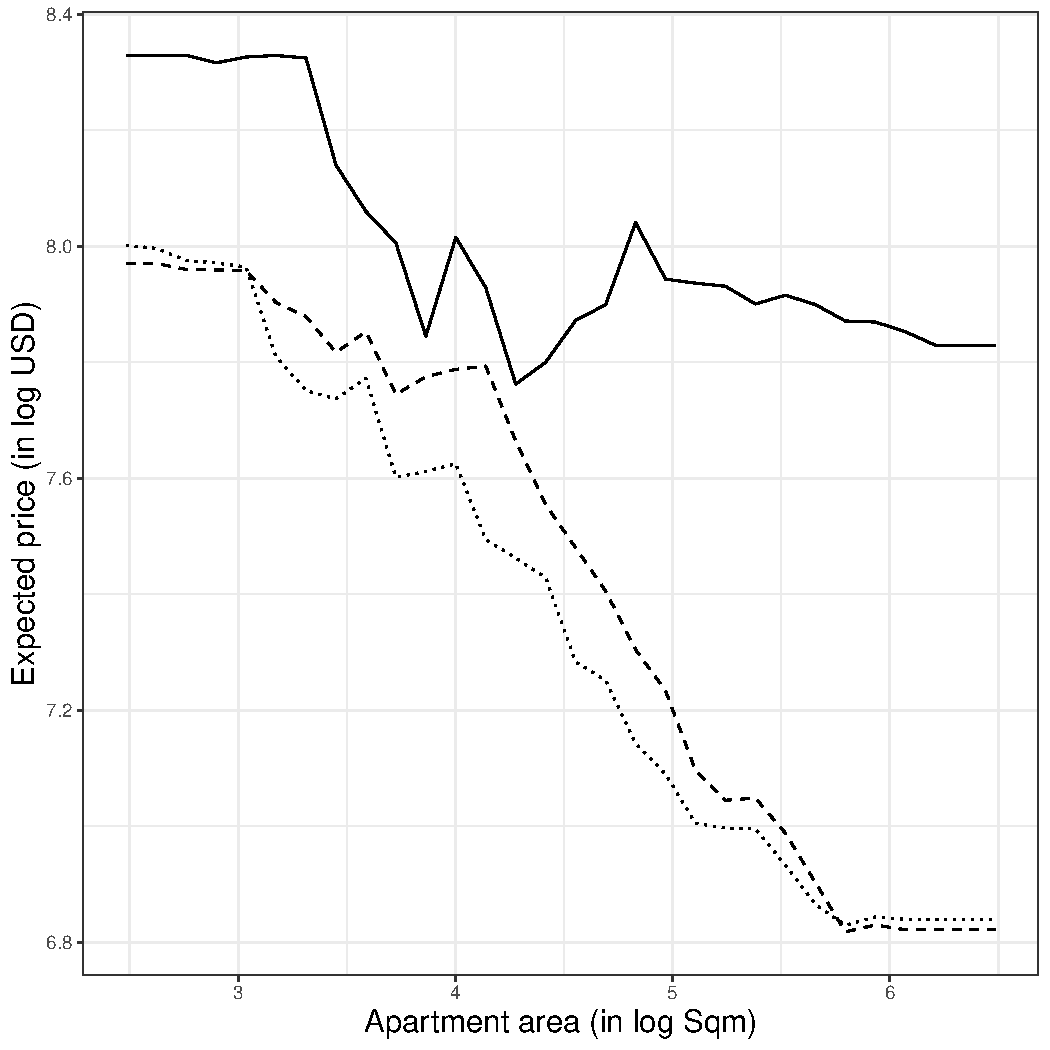
\includegraphics[scale=.5]{figures/fig-3ice-exmp.pdf}
    \caption{Individual ICE curves, where each line represents one selected observation.}
    \label{fig-3ice} 
\end{figure}
%\includegraphics[trim=0cm 4cm 0cm 4cm, clip, scale=1]

\subsection{Spatial ICE (SpICE) curves} 
\label{seccD}

The interpretation of ICE curves can be challenging when a large number of observations is available. A solution based on clustering ICE curves, which takes into account two sources of information, is proposed. The main source of information corresponds to the covariate effect profile described by the ICE curve itself. This is relevant to maintaining the original goal of the individual ICE curves. Additionally, when observations contain individual spatial information, location information can be used to improve the interpretability of ICE curves. Spatial data is data where the location of the measurements is a key element. This often includes data that references a specific geographical area. In this paper, SpICE refers to clustering ICE curves with spatial contiguity constraints.

In order to construct clusters of ICE curves, it is necessary to define a distance or dissimilarity measure between functions. There are many approaches that can be used to solve this problem; a typically used metric for functional clustering is the L2 distance: 
\[ d_{L2}(i, j) = \sqrt{ \int |\hat{f}_{S}^{(i)}(x) - \hat{f}_{S}^{(j)}(x)|^2dx}, \] 
where $d_{L2}(i, j)$ represents the L2 distance between ICE curve $i$ and ICE curve $j$. In Appendix \ref{toyexample}, a model example in which the L2 distance is not adequate to distinguish ICE curves with different predictor effects profiles is presented. Figure \ref{iceej} presents two scenarios in which $d_{L2}(\cdot,\cdot)$ produces the same value but the covariate effect is not the same. 

Moreover, \cite{hitchcock2015clustering} point out that in many applications, information about the derivatives of the function is even more relevant than the function itself.  In these cases, one approach could be to use the same L2 distance on the derivative functions. However, in clustering ICE curves, the key idea is to group observations with similar predictor effects on the response; thus, considering both the level and variation is important. For these reasons, it is appropriate to consider a distance that takes into account not only the value of the function but also its growth/decrease. Therefore, for the ICE function $\hat{f}_{S}^{(i)}(x_S)$, it is possible to use the Sobolev $W^{1,2}(\mathbb{R})$ distance \citep{sobolev}:  
\begin{equation}
\label{sobodis}
d_{Sob}(i, j) = \sqrt{ \int |\hat{f}_{S}^{(i)}(x) - \hat{f}_{S}^{(j)}(x)|^2dx + \int |\hat{f^{'}}_{S}^{(i)}(x) - \hat{f^{'}}_{S}^{(j)}(x)|^2dx}.    
\end{equation}  

The Sobolev distance has recently been used in some functional data applications as a way to highlight complex functional patterns. \cite{cremona2023probabilistic} and \cite{ehsani2020robust} report good performances when this type of distance is used in different statistical applications. Particularly in clustering functional data, using the Sobolev distance might improve the clustering solution. In Appendix \ref{simstudy}, results from a small simulation study are presented.  A classical functional data example \citep{hitchcock2007effect} is used to compare the proportions of correctly matched pairs of curves when the L2 or Sobolev distance is used. The Sobolev distance shows better results in at least 95\% of the 500 replications.   

However, some statistical learning models (such as tree-based methods) produce nondifferentiable predictor functions; thus, the ICE curves for these models inherit the nondifferentiability property, which makes the computation of $d_{Sob}(,)$ impossible. One way to overcome this issue and obtain estimates in a $C^1$ space is to consider the curve $\widetilde{f}_{S,ICE}^{(i)}(x_S)$, which is the convolution of the function  $\hat{f}(x_S, x_C^{(i)})$  with a Gaussian kernel. That is, 
\begin{equation}\label{}
 \widetilde{f}_{S}^{(i)}(x_S) := \ \hat{f}(x_S, x_C^{(i)}) \ast K_h(x_S),
\end{equation}
where $K_h$ is the Gaussian kernel, $h$ is the smoothing parameter and $\ast$ is the convolution operation. It is worth noting that this operation can be thought of as a pre-smoothing of the functional data, which has been shown to be beneficial in the cluster analysis of functions \citep{hitchcock2007effect}. Additionally, when the true $f(x)$ is a smooth function, the above transformation of the ICE curve (the convolution) will not distort the ICE estimator in a relevant way. 

When considering ICE curves, each curve is associated with a specific observation. In applications in which the location is a key element, i.e. spatial problems, it is possible to link such curves with the location information of the corresponding observation. Combining these two sources of information might improve the interpretability of ICE curves. 

\cite{chavent2018} propose an algorithm to construct clusters of multivariate data with spatial restrictions of contiguity. 
Let us consider a partition $\mathcal{P}_K = (C_1 ,\ldots , C_K )$ into $K$ clusters.  Using two dissimilarity matrices, $D_0$ and $D_1$, and a mixing parameter $\alpha \in [0,1]$, the pseudo-inertia in cluster $k$ can be defined as 
$$I_{\alpha} \left( C^{\alpha} _k \right)=  (1-\alpha) \sum_{i \in C^{\alpha}_k} \sum_{j \in C^{\alpha}_k} d^2_{0,ij}+\alpha \sum_{i \in C^{\alpha}_k} \sum_{j \in C^{\alpha}_k}d^2_{1,ij},$$
where $d_{0,ij}$ and $d_{1,ij}$ represent dissimilarities between observations $i$ and $j$ in $D_0$ and $D_1$, respectively. Then, a Ward-like method \citep{ward1963hierarchical} is used for the construction of the clusters, and a data-driven procedure to assist in the choice of the $\alpha$ value is proposed. 

In this paper, this clustering algorithm is adapted to cluster ICE curves (functional data). Mainly, the dissimilarity matrix $D_0$ represents distances among ICE curves instead of multivariate data. The Sobolev distance is used to compute dissimilarities among pre-smoothed ICE curves and to construct the $D_0$ matrix, i.e $d_{0,ij} = d_{sob}(i, j)$ (see Equation \eqref{sobodis}). As mentioned earlier, this distance takes into account the covariate effect profile in terms of both the level and variation and could be beneficial for the clustering solution. In addition to ICE information, the geographical distance between 
observations is used for the $D_1$ matrix. The \texttt{SpICE} R package implements the computation and visualisation of SpICE curves; it is available at  https://github.com/natydasilva/SpICE. 


\section{Application results}
\label{section:appl}

\subsection{Dataset: Apartment prices in Montevideo}
The data in this paper are from an eCommerce platform called \href{https://www.mercadolibre.com.uy)}{Mercado Libre}, where apartments and houses are offered for sale and for rent. The complete dataset contains asking price information for properties in Montevideo, the capital city of Uruguay, from February 2018 to January 2019 \citep{Picardo}. There are 92,832 observations; however, only apartment data will be considered for the analysis, which results in 70,817 observations concerning apartments for sale in Montevideo.

 Figure \ref{mapa} shows the distribution of the asking price for apartments in Montevideo, where each dot represents one apartment for sale and the colour represents the asking price of the apartment per square metre in US dollars. Figure \ref{mapa} suggests that locations close to the coast are associated with a higher price range. The asking price ranges from 541 to 5,000 US dollars per square metre in Montevideo, and the median value is close to 2,500 US dollars.  
 \begin{figure}[hbpt]
\centering
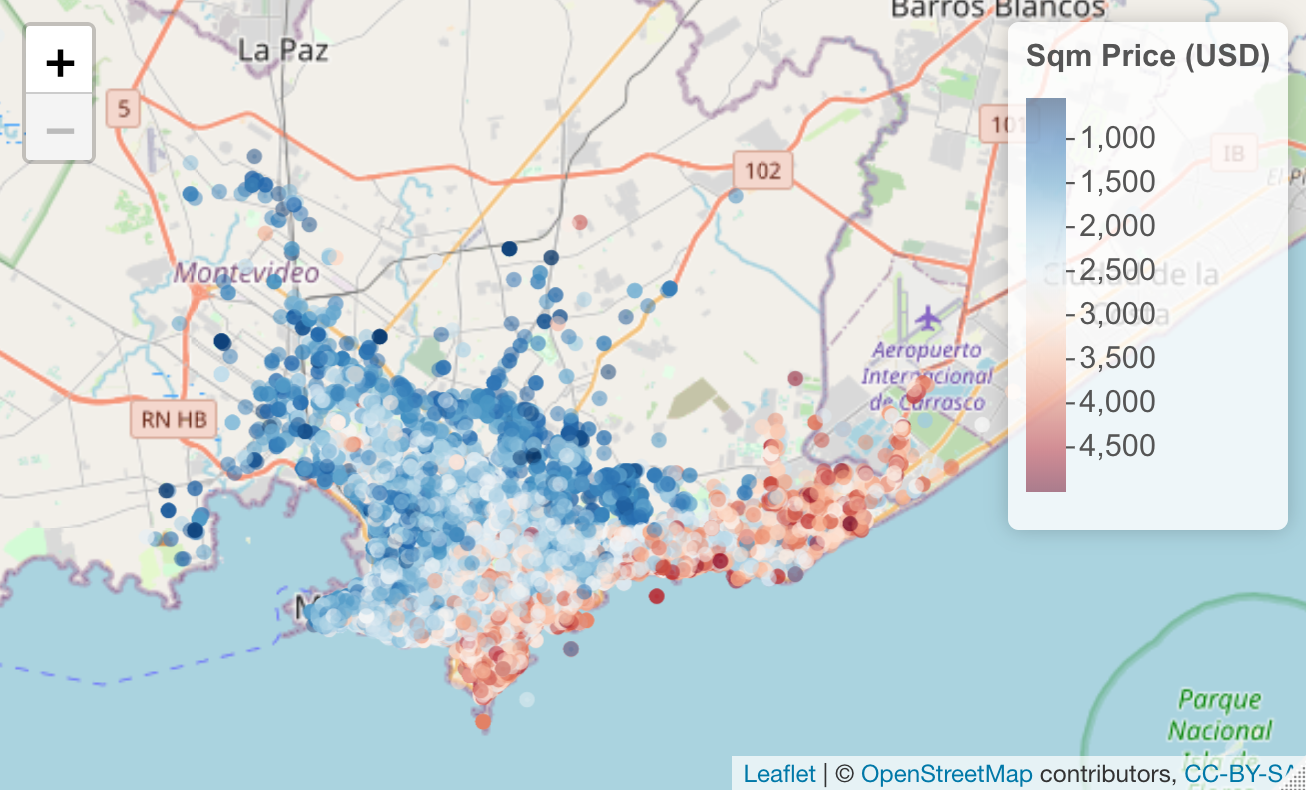
\includegraphics[width=1\linewidth]{figures/mapa_preciom2.png}
\caption{Distribution of the asking price for apartments in Montevideo. Each dot represents one apartment, and the colour represents the asking price offered by the seller in US dollars per square metre. 
\label{mapa} }
\end{figure}

\begin{table}[hbpt]
	\centering
	\caption{Variable description\label{tabvar} }
\scriptsize
\begin{tabular}{p{2.4cm}p{7cm}}
		\hline \\[-1.8ex] 
\textbf{Variable} &  	\textbf{Description} \\
		\hline \\[-1.8ex] 	\hline \\[-1.8ex] 

\texttt{lpricem2}  & Log of asking price in US dollars per square metre. \\ \hline
  
\texttt{amenities}  & Total number of amenities present in the apartment.\\
\texttt{bedroom}  & Bedroom quantity. Reduced to values between 0 (studio) and 3. \\
\texttt{bathroom}  & Bathroom quantity. Reduced to values between 1 and 3.\\
\texttt{elevators}  & Elevator quantity. Reduced to values between 0 and 2. \\
\texttt{condition}  & Property condition (new/used).  Properties that were less than 1 year old were marked as `new'.\\
\texttt{expenses}  &  Numerical value representing monthly expenses in Uruguayan pesos (local currency).\\
\texttt{garage}  & Whether or not there is a garage. Reduced to values between 0 (`No') and 1 (`Yes').\\ 
\texttt{ldistance\_beach}  & Minimum distance (Euclidean)  between  the property   and the beach (on a log scale). \\
\texttt{larea\_apt}  & Log of the apartment area in square metres. Values over 2,000 or under 9 square metres were removed from the data. \\
\texttt{neighborhoodgr}  &  Montevideo neighbourhoods grouped by proximity in 12 regions. \\ \hline
\texttt{lat} & Property latitude coordinate. \\
\texttt{long}  & Property longitude coordinate. \\
	\hline \\[-1.8ex] 	\hline \\[-1.8ex]  
	\end{tabular}
\end{table}

The complete dataset contains 116 explanatory variables representing apartment features commonly used in real estate modelling. With the available information, an additional two explanatory variables were created. First, a variable indicating the distance from the apartment to the beach was computed since it appears to be a relevant feature based on data exploration (see Figure \ref{mapa}). Second, many of the variables indicate the presence/absence of one specific amenity; thus, a variable indicating the total number of amenities present in an apartment was computed. 

A reduced number of variables were selected to improve the data quality of the complete dataset. Table \ref{tabvar} presents the selected variables, indicating the name of each variable in the dataset and a brief description. All the models were fitted using the natural logarithm of the  price per square metre (\texttt{lpricem2}) as the response variable. Finally, the geographical coordinates of each property were not used as explanatory variables in the models but were used as additional information to improve interpretability using the SpICE curves described earlier.
 
\subsection{Predictive models}
\label{modelo} 

Several models were trained %to estimate $f(x_i)$ 
using the automatic machine learning (\texttt{autoML}) procedure from the \texttt{h2o} R package \citep{h2o} to predict the apartment  price as an alternative to classical methods. \texttt{autoML} estimates well-tuned models in four families: penalised linear models (glm), random forest (drf), extreme gradient boosting (xgboost) and fully connected multi-layer artificial neural networks (deeplearning). Additionally,  stacked ensembles (stackedensemble) of individual models are trained; this includes the combination of all the models and ensembles using subsets of trained models. In the rest of the paper, the best model of each family and the best-performing stacked ensemble are used. 

Table \ref{comparo} shows the  performance measures for the selected predictive models.  The root mean square error (RMSE) and the $R^2$ value are used to evaluate the model performance. These values are computed with the response variable in logs (as this was done for the training of every model). Additionally, the mean absolute error (MAEo) and mean absolute percentage error (MAPEo) are both computed on the original scale of the response variable, so they have units of dollars per square metre.  The four measures are computed using a testing dataset different from the training samples (2/3 training and 1/3 testing). 

\begin{table}[ht]
\centering
\caption{Predictive performance measures by model} 
\label{comparo}
\begin{tabular}{rlrrrr}
  \hline
 & model & rMSE & R2 & MAEo & MAPEo \\ 
  \hline
1 & stackedensemble & 0.14 & 0.81 & 242.68 & 9.58 \\ 
  2 & drf & 0.14 & 0.80 & 251.08 & 9.94 \\ 
  3 & xgboost & 0.15 & 0.80 & 254.48 & 10.06 \\ 
  4 & deeplearning & 0.20 & 0.63 & 395.84 & 15.18 \\ 
  5 & glm & 0.22 & 0.55 & 427.72 & 17.13 \\ 
   \hline
\end{tabular}
\end{table}

In terms of the predictive performance, the stacked ensemble, random forest and xgboost algorithms show similar performances; they are somewhat better than the deep learning method or the penalised linear model. It is worth noting that the stacked model combines seven tree-based models. The best model obtained an average error in the asking price of \$243 per square metre, or around 9.6\% of the observed price.  %The variability explained by  every model is between $0.74$ and $0.90$. 

\subsection{Variable importance measures}
\label{sec:varimp} 
The first approach to interpreting model results for statistical learning methods is to compute variable importance measures. 
The variable importance measures were scaled so that the most important variable in each model has a value of 1, which simplifies the model comparison.  In Figure \ref{fig-imp}, we show  the results  by model for the variable importance. The ordering of the predictors is similar in all models. The apartment area (\texttt{larea\_apt}) and the neighbourhood (\texttt{neighborhoodgr}) are the two most important variables for predicting the apartment price. All the tree-based methods (drf, xgboost and stackedensemble) show a third relevant variable, which is the distance from the apartment to the beach (\texttt{ldistance\_beach}). The rest of the predictor variables are not relevant for prediction.  

\begin{figure}[htpb]
    \centering
    %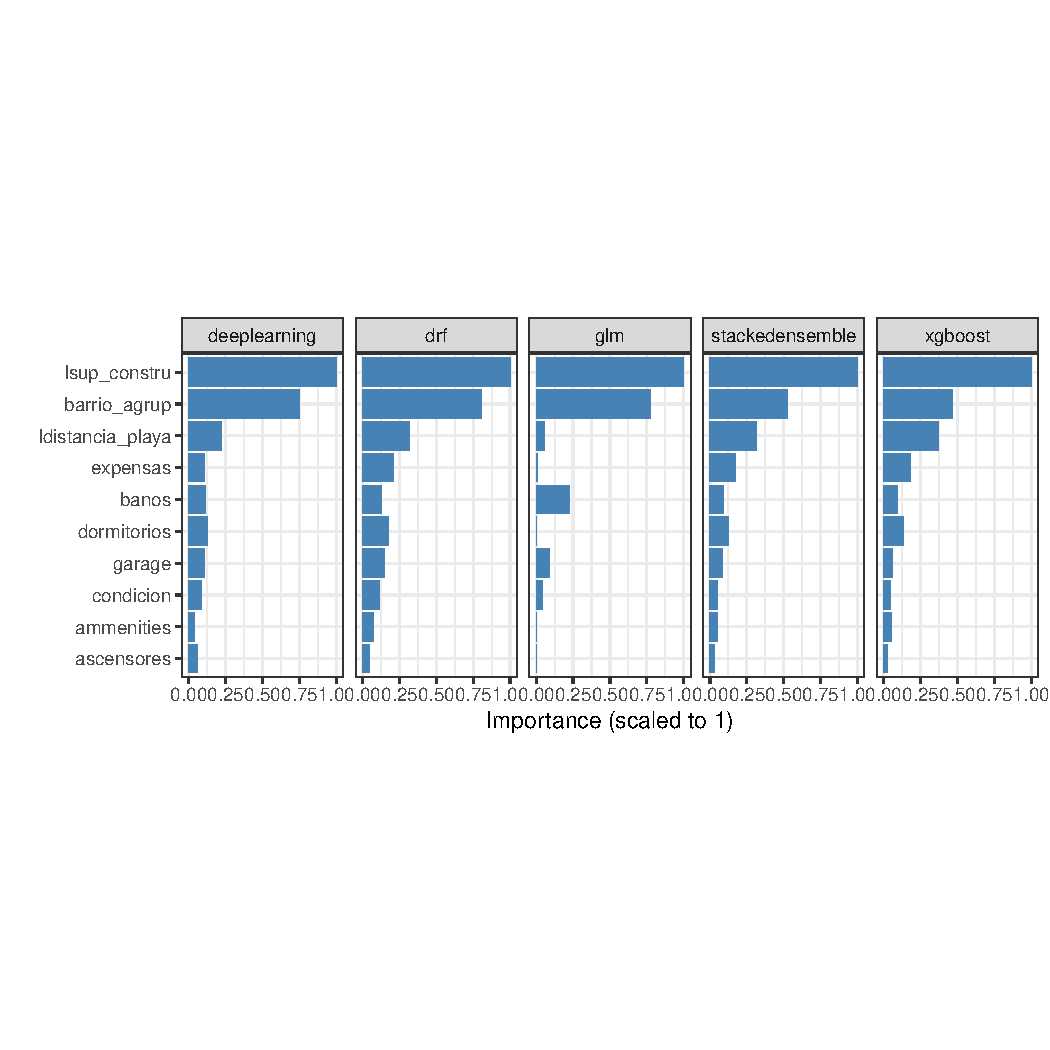
\includegraphics[trim=0cm 4cm 0cm 4cm, clip, scale=1]{figures/fig-importance.pdf}
    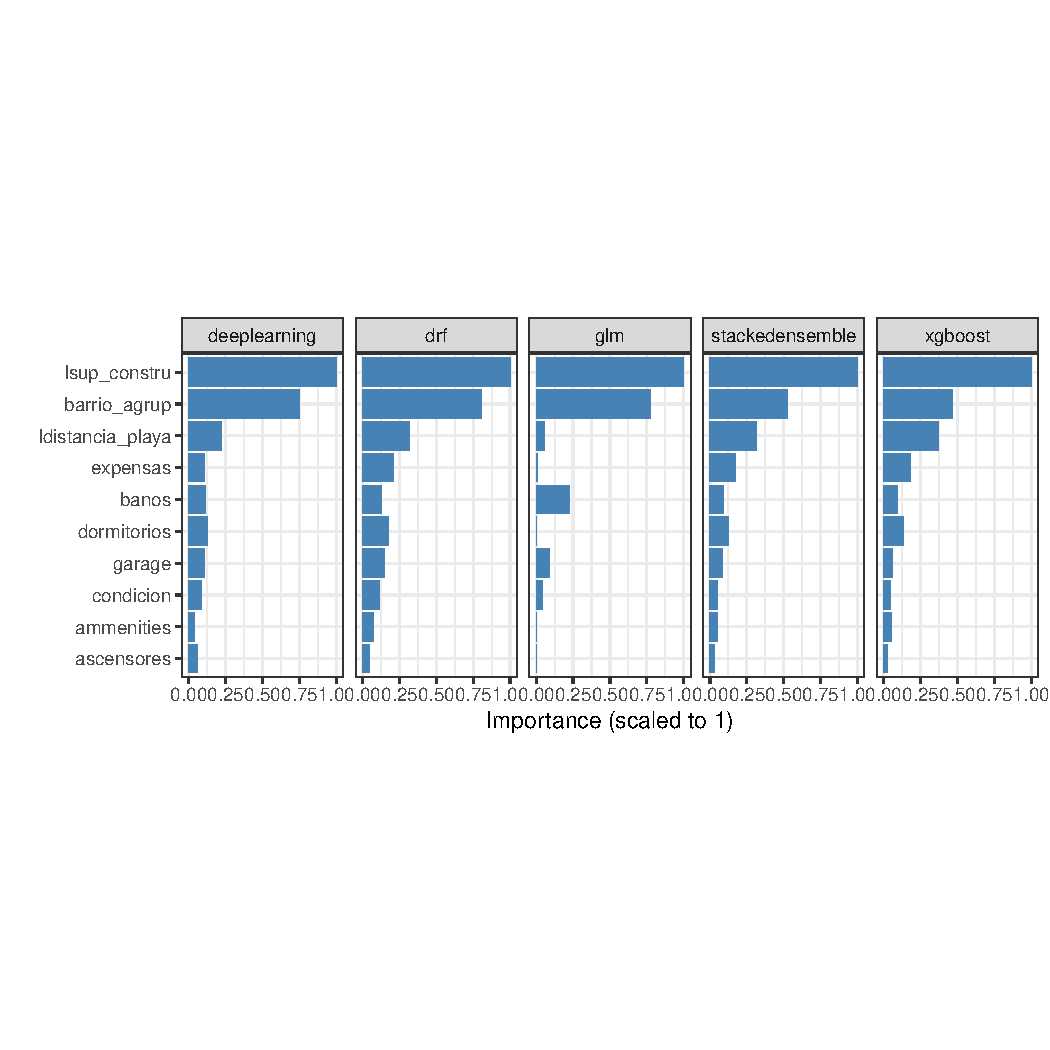
\includegraphics[scale=.9]{figures/fig-importance.pdf}
    \caption{Variable importance. Each panel represents a model, and the y-axis shows the variables included in all the models. The bar length represents the scaled variable importance measure used to predict the apartment price.}
    \label{fig-imp}
\end{figure}

\subsection{Partial effect of apartment area} \label{sub:resultados_pdp}
In subsection \ref{sec:varimp}, the variable importance was presented; these results provide a ranking of variables according to their relevance for predicting the response variable.  However, they do not provide information on the effect that the individual variables have on the response variable. In order to characterise the average effect of apartment features on the price, the PD-plot and the ALE-plot  are estimated. The algorithms used for this estimation are from the R packages \texttt{pdp} \citep{pdp} and \texttt{ALEPlot} \citep{aleplot}. 
%interpretable methods described in Section \ref{section:2} are computed. Computations of the PD-plot, ALE-plot and ICE curves are done using R packages \texttt{iml} \citep{iml} and \texttt{ALEPlot} \citep{aleplot}. 
\begin{figure}[hbpt]
    \centering
    %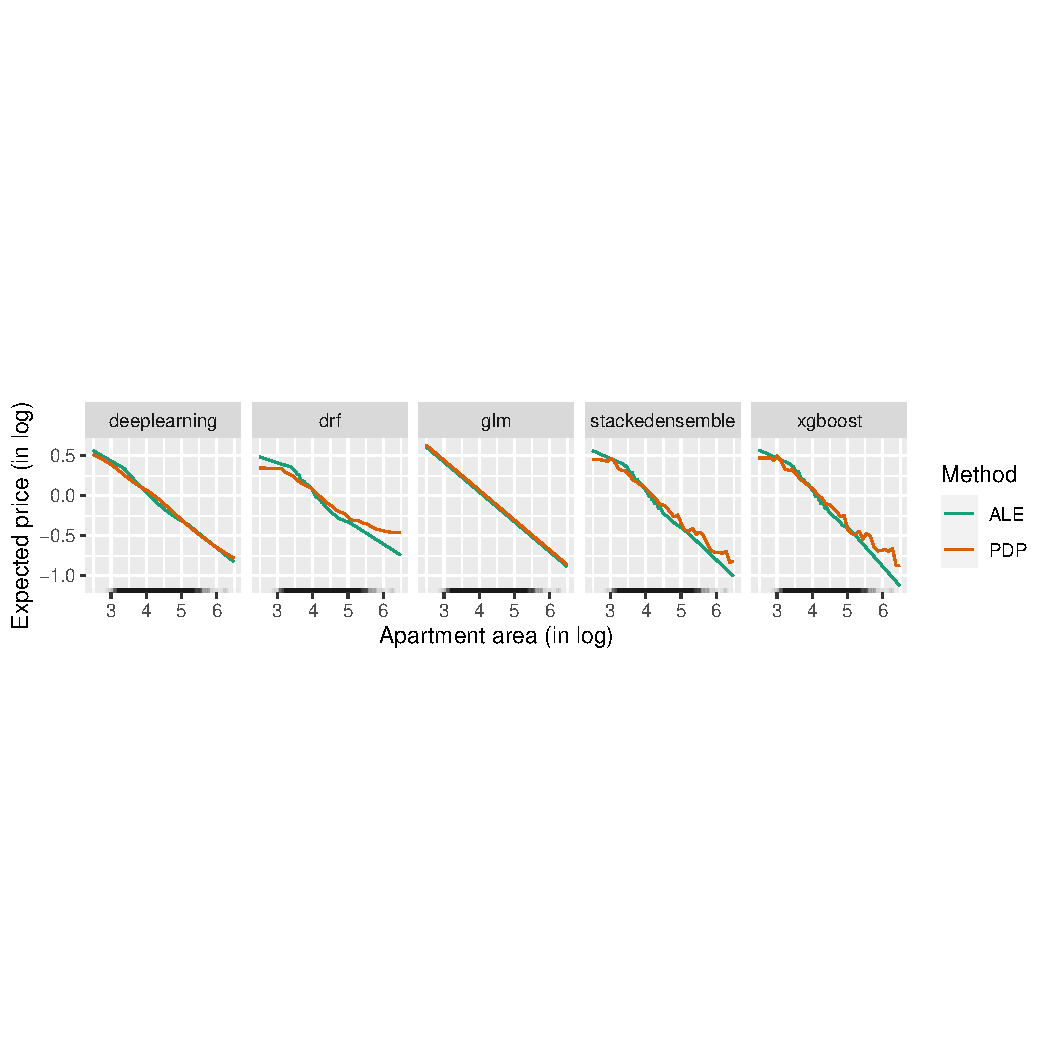
\includegraphics[trim=0cm 6cm 0cm 6cm, clip, scale=1]{figures/fig-efecto-lsub.pdf}
    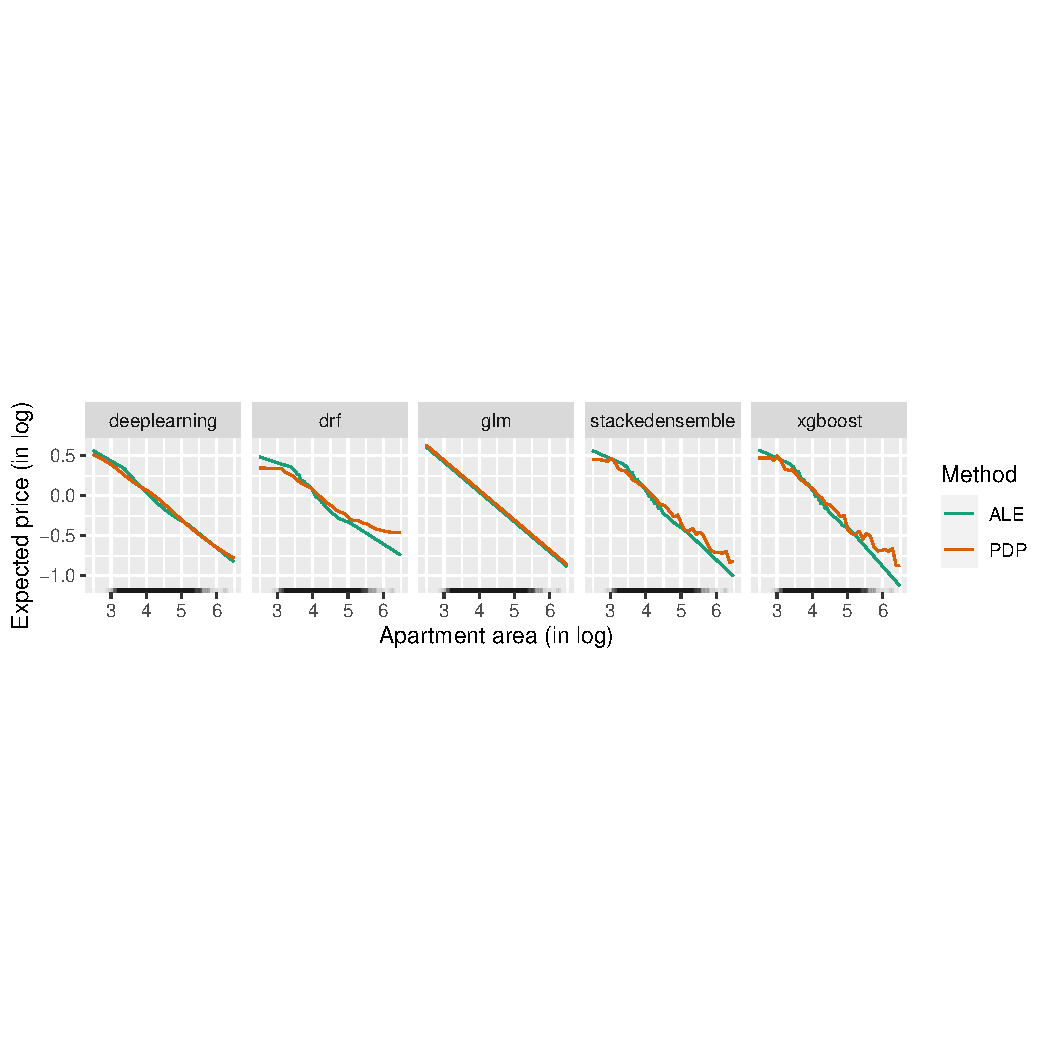
\includegraphics[scale=.9]{figures/fig-efecto-lsub.pdf}
    \caption{Effect of the \texttt{larea\_apt} variable in different models. Each panel corresponds to a predictive model and the colour represents the interpretable method (ALE-plot or PD-plot).}
    \label{fig-pdpalesup}
\end{figure}

The apartment area (\texttt{larea\_apt}) is the most relevant feature in every model. The effect of this variable on the response is described with the PD-plots and ALE-plots shown in Figure \ref{fig-pdpalesup}, where each panel corresponds to a model. A negative effect is suggested by these plots, with a similar effect in every model. Especially, this is  true  in the middle of the range for the apartment area, where most of the observed samples lie. Some differences can be seen in very large or very small apartments, where random forest shows smaller effects on prices. 

Specifically, Figure \ref{fig-pdpalesup} shows the average effects of the variable \texttt{larea\_apt}  in the sample. In a scenario in which the impact of an explanatory variable on the response presents heterogeneity among the observations, the PD-plot and ALE-plot methods hide the variability of effects. An alternative method for interpretability that can be used to tackle this issue is the ICE-plot. The value of visualising the individual curves that compose the PD-plot lies in exploring other patterns in the effects, rather than just the mean value.  

When big datasets are involved, a major disadvantage of ICE-plots is overplotting, which makes it difficult to answer  anything. This is especially relevant for ICE curves since their main purpose is to look for heterogeneity patterns in the predictor effect. The use of graphical solutions such as transparency or 2-dimensional histograms is not suitable for plotting lines.  In the \texttt{h2o} implementation (\cite{hall2017}), a few ICE curves for decile values (in the observed response) are displayed, so no matter how large the sample data are, only ten ICE curves are displayed, resulting in an oversimplified plot. An alternative is to plot a stratified sample of curves. This method can be combined with line transparency to allow one to reduce overplotting while making it possible to see the different patterns of the ICE curves in the data. Figure \ref{fig-icesupRF} shows the individual conditional expectation plot for the apartment area (\texttt{larea\_apt}) for the  random forest model. The other predictive models shows similar results, as can be seen in Figure \ref{fig-icesup} in Appendix \ref{app:figsup}. 

\begin{figure} 
    \centering
    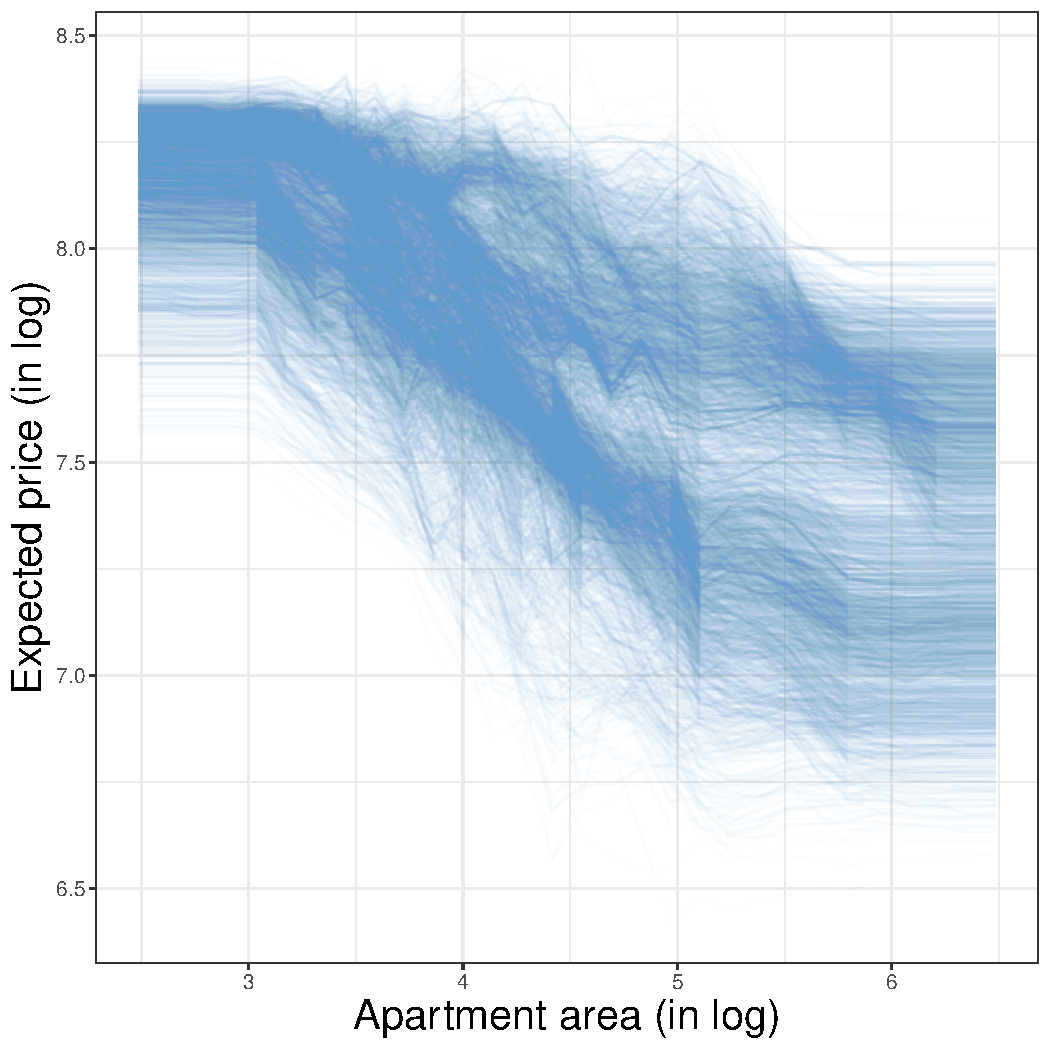
\includegraphics[scale=0.5]{figures/fig-ice-sup-decRF.pdf}
    \caption{ICE-plot for the \texttt{larea\_apt} variable. Each panel corresponds to a predictive model. Five thousand randomly stratified selected curves are shown.}
    \label{fig-icesupRF}
\end{figure}

The results illustrate the negative effect of the variable \texttt{larea\_apt} in each individual curve. However, it is relevant to note that the effect  presents  heterogeneity for the different properties. Figure \ref{fig-icesupRF} suggests that for properties with a high predicted price, the apartment area presents a small and linear effect, while cheap properties show a non-linear and larger impact of the apartment area. 

\subsection{SpICE curve effects} \label{results-ice}
Finally, to explore the connections among ICE curves and the geographical locations of properties, the SpICE curve results are presented.  
A range of three to five clusters is considered; for each value, an optimal value for the $\alpha$ parameter is determined as a compromise between the internal homogeneity of the clusters in terms of the ICE curves and the geographical information, approximately. The results are shown in Figure \ref{alpfaoptimo} in Appendix \ref{app:figsup}, using four groups and $\alpha = 0.5$.

Figure \ref{fig-spice} show the results of the geographically constrained clusters; an apartment for sale in Montevideo is represented as a point on the map that is linked to an ICE curve in the bottom panel. The colours of the points and curves indicate the cluster that they belong to. The cluster locations suggest a layout in the north-west/south-east direction, similar to the price gradient present in the data (see Figure \ref{mapa}). The apartments in the west and on the north-west side (green cluster) correspond to low-income neighbourhoods, while the east side of the city (red cluster) represents the zone with the highest income in Montevideo. 

Focusing on the SpICE curves presented in Figure \ref{fig-spice}, there are distinct patterns in the relationship between the apartment area and the asking price per square metre. Across all clusters, there is a negative relationship between the price per square metre and the apartment area. However, the effect of the apartment area on the price per square metre differs between the green and blue clusters (associated with medium- and low-income neighbourhoods) and the red and violet clusters (associated with high-income neighbourhoods). In the red and violet clusters, an increase in the apartment area results in a smaller decrease in the price per square metre compared to the green and blue clusters. This suggests that, in high-income neighbourhoods, the total apartment price (not the price per square metre) is very sensitive to changes in the apartment area. Conversely, in low-income neighbourhoods, the total apartment price is inelastic to changes in the apartment area. Consequently, additional square metres in the apartment have no impact on the total apartment price, leading to a decline in the price per square metre. %within the low and medium-income neighborhoods.


\begin{figure} 
    \centering
    %{figures/fig-4grupos.pdf}
    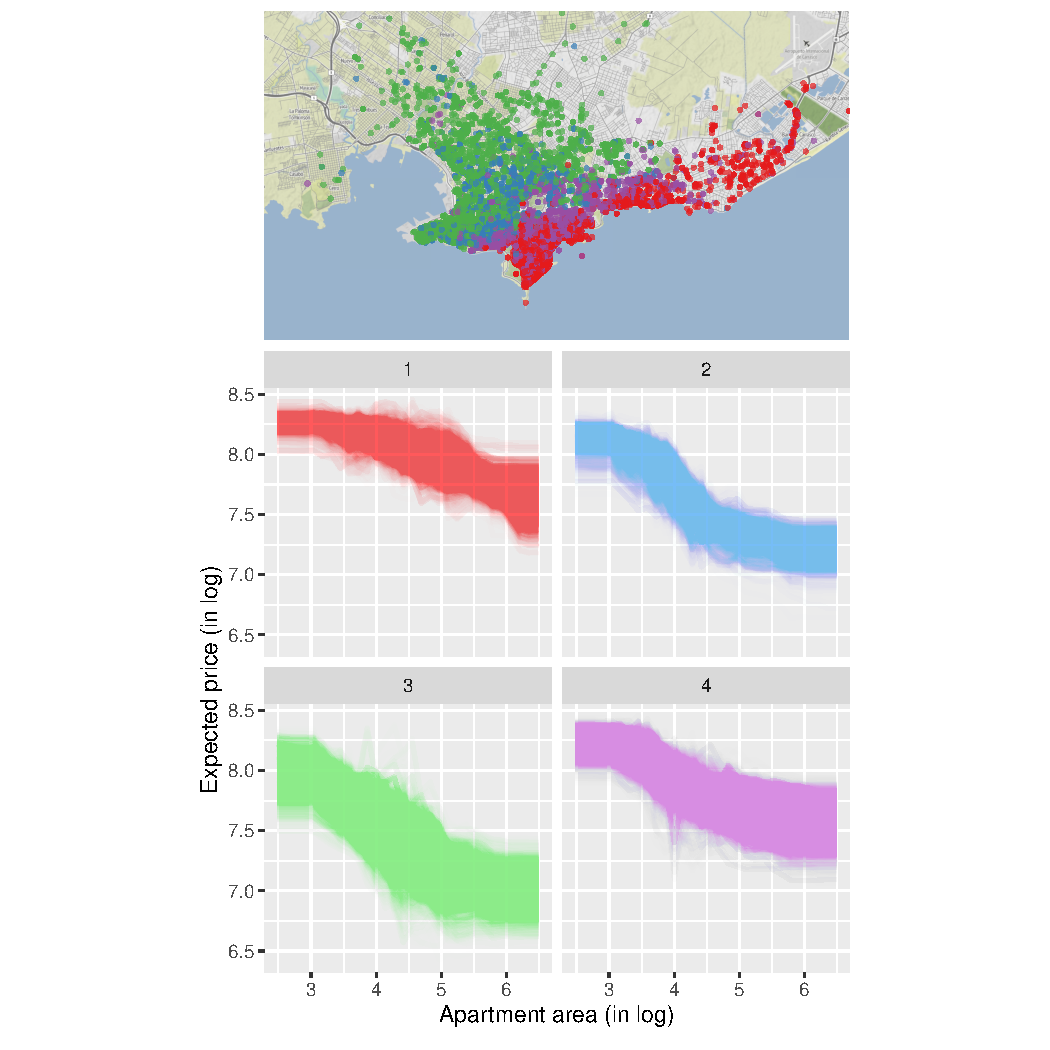
\includegraphics[scale=0.9]{figures/fig-4grupos-alpha5.pdf}
    \caption{SpICE curves and geographical locations of clusters.}
    \label{fig-spice}
\end{figure}



\section{Discussion} \label{section:4}

In this paper, interpretable methods for measuring heterogeneous covariate effects for black box models, functional data clustering and spatial information were combined to improve interpretability in spatial applications. In particular, geographically constrained clusters of ICE curves called SpICE curves were constructed, combining two sources of information.  On the one hand, the covariate effect profile is considered by using the Sobolev distance as a dissimilarity measure for the ICE curves. The Sobolev distance is useful from an interpretability point of view since it summarises the main characteristics of the covariate effect (level and variation). On the other hand, the location information of observations is used to obtain geographically contiguous clusters. 

Similarly to the ICE-plot, the SpICE curves can show the heterogeneous effects of a predictor variable in a black box model. SpICE curves are easier to work with in big data applications since it is possible to interpret each cluster instead of each individual curve. In specific problems, the spatial contiguity of the cluster provides more interpretable information associated with other relevant aspects that may not be present in the ICE curves. 

In the motivating example, SpICE curves were constructed to profile the effect of the total area of a property on the  price per square metre in Montevideo apartments. Five statistical learning methods were selected from a list of fitted models using \texttt{h2o} with the \texttt{autoML} procedure based on the predictive performance. The predictor variable `total area of the apartment' was (unsurprisingly) the most important feature in  all models. Then, using a fitted model with the random forest algorithm, the ICE-plot and SpICE curves for each apartment were computed. The spatial information of the properties was combined with ICE curves to gain interpretability. Four property clusters were selected, based on a distance that combines the functional distance between ICE curves and the geographical distance between apartment coordinates.  The blue and green clusters mainly represent properties located in medium- or low-income zones in Montevideo, and these clusters present a large, negative, non-linear effect of the apartment area on the price per square metre. On the other hand, the red and violet clusters mainly correspond to high-income neighbourhoods, and they show a small, close-to-linear effect of the property area. 

There are several aspects of this paper that could be explored in future work. First, the choice of the distance between the ICE curves could be improved; specifically, it is relevant to analyse more deeply in which scenarios the Sobolev distance results in a better clustering solution for functional data.  Second, instead of constructing fixed clusters of ICE curves, it is possible to consider the local average of the ICE curves in a nearest neighbours fashion, where the distance used to determine the neighbours could combine the structure of the ICE curves and the geographical distance. Finally, a summary of the clustered ICE curves could be based on the ALE-plot instead of the average of the clustered ICE curves. 

\section{ Supplementary material }
This article was written with the R packages \texttt{knitr} \citep{knitr}, \texttt{ggplot2} \citep{hadley:2016}, \texttt{leaflet} \citep{leaflet}, \texttt{tidyverse} \citep{tidyverse}, \texttt{h2o} \citep{h2o}, \texttt{ClustGeo} \citep{clustGeo} and
 \texttt{KernSmooth} \citep{KernSmooth}. The files needed to reproduce the article and the results are available at https://github.com/natydasilva/SpICE\_COST. Additionally, the \texttt{SpICE} R package implements the computation and visualisation of SpICE curves proposed in this paper and  it is available at  https://github.com/natydasilva/SpICE. 





\renewcommand{\refname}{References }
\bibliographystyle{chicago}
\bibliography{bibcsic.bib}


\appendix

\section{Minimal example \label{toyexample}}  
This section presents a model example in which the L2 distance is not a good choice for finding dissimilarities among ICE curves. Let us assume the regression model 
\[\begin{array}{cl}
  Y_i   &  = f(X_{1,i}, X_{2,i}) + \epsilon_i  \\
     & = -C(1-X_{1,i})X_{1,i} + \frac{1}{2}X_{2,i}(2- X_{1,i}-X^2_{1,i}) +X_{2,i}^{1+X_{1,i} \mathds{1}{ \{X_{1,i}\geq 0\} } }  + \epsilon_i,
\end{array}\]

where $X_1 \sim U(-1,1)$, $X_2\sim U(0,2)$ and $\epsilon_i$ represents white noise with a standard deviation $\sigma>0$. When the true $f()$ function is known, the ICE curves at three chosen points are $f(-1,x2)= 2C+2x_2$, $f(0,x2)=2x_2$ and $f(1,x2)=x_2^2$. If $C= -\sqrt{ \frac{\int_0^2(x^2-2x)^2 dx}{8}}$, then 
$$d_2\left( f(-1,\cdot), f(0,\cdot)\right)= d_2\left( f(1,\cdot), f(0,\cdot)\right).$$

Figure \ref{iceej} shows these three ICE curves in two panels. The left panel (case 1) contains $f(-1,\cdot)$ and $f(0,\cdot)$, two parallel linear functions representing the same effect of $X2$ on the response variable. Meanwhile, the right panel (case 2) shows the ICE curves for $f(1,\cdot)$ and $f(0,\cdot)$; here, the two curves represent different effects of $X2$. 

\begin{figure}[hbpt]
\centering
%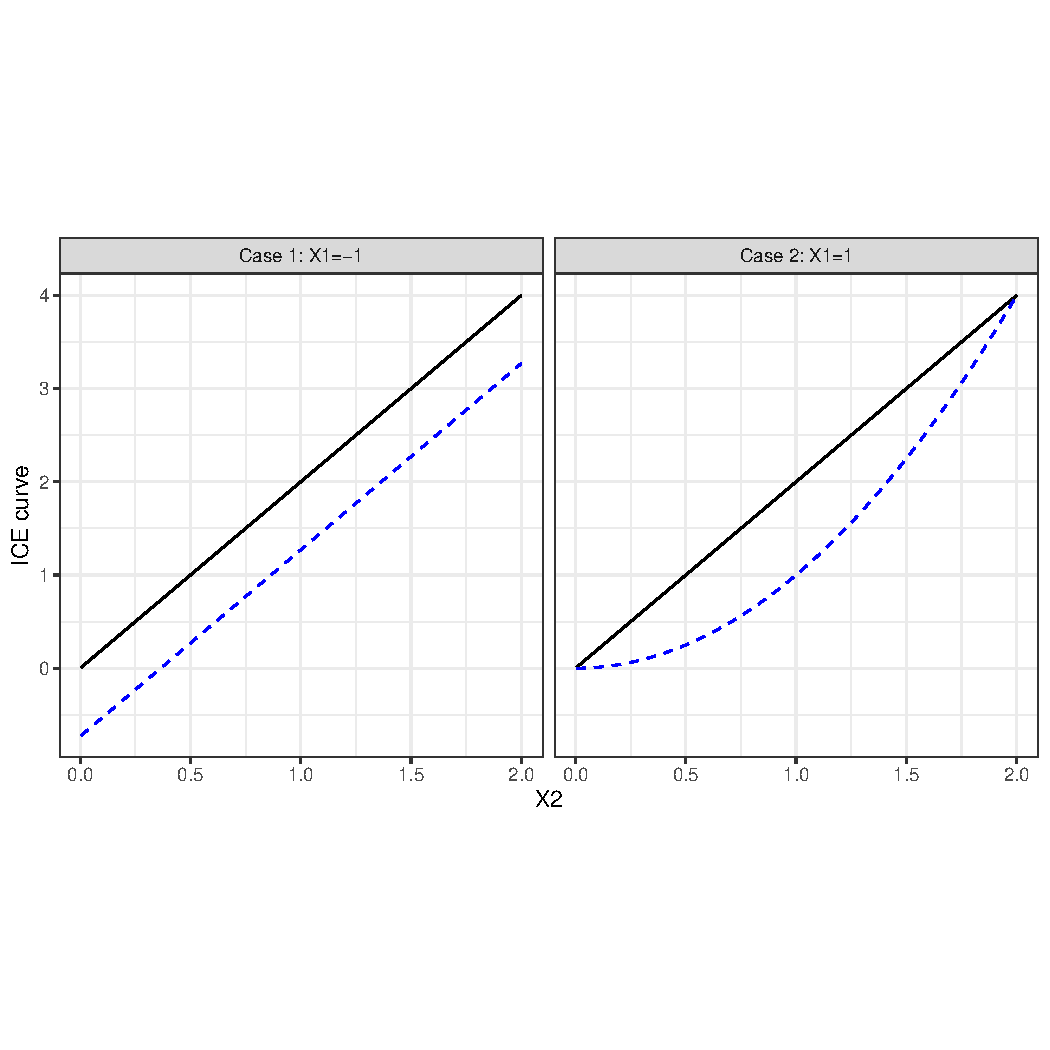
\includegraphics[height=4cm,  width=1\linewidth]{figures/fig-toyexample.pdf}
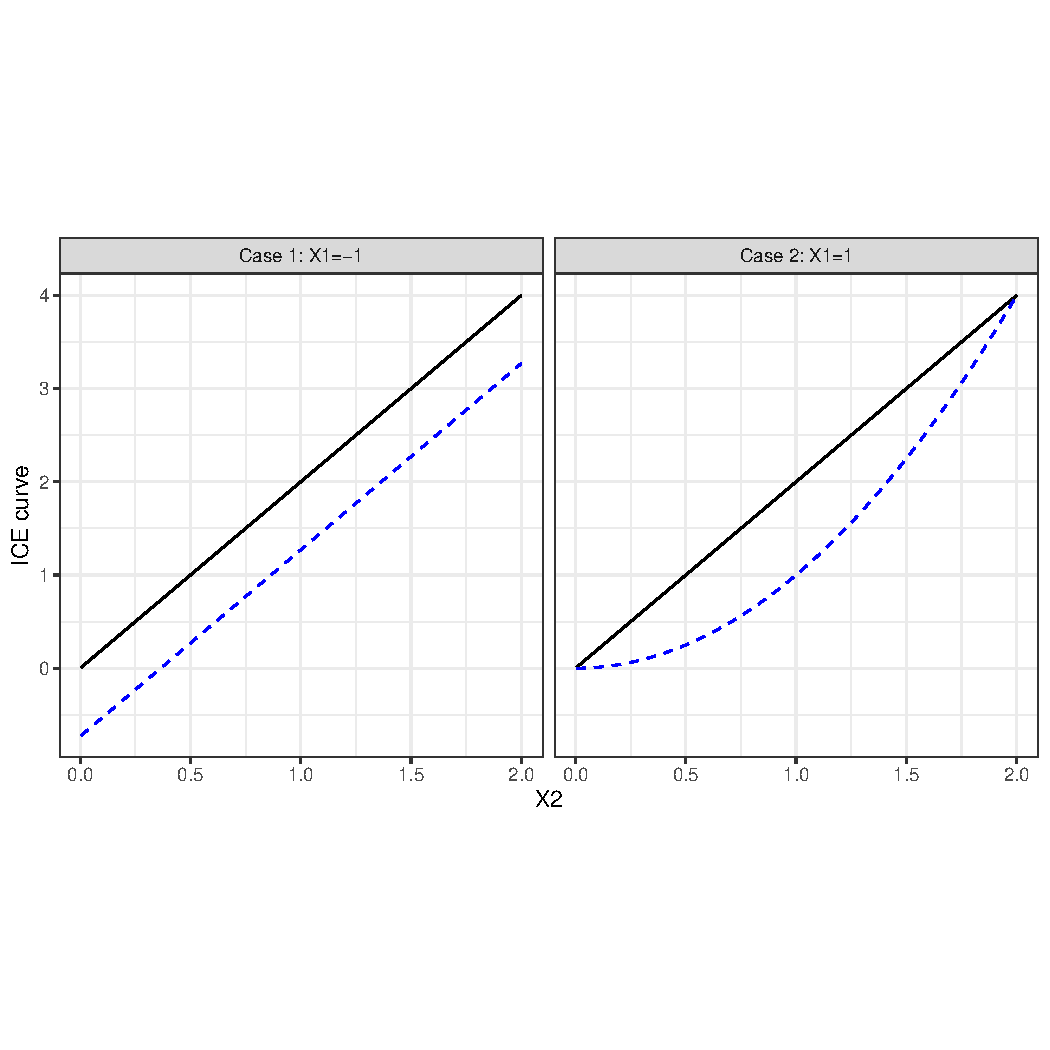
\includegraphics[trim=0cm 4cm 0cm 3cm, clip, scale=.7]{figures/fig-toyexample.pdf}
\caption{ICE curves from the model example. \label{iceej} }
\end{figure}
From an interpretability point of view, it is important to differentiate between the two cases plotted in Figure \ref{iceej}; however, the L2 distance is the same in these two cases. 

\section{Simulation study \label{simstudy}}

A small simulation study comparing the performances of the L2 and Sobolev distances in clustering functional data is performed, following the design choices proposed in \cite{hitchcock2007effect}. 
\begin{figure}[hbpt]
\centering
%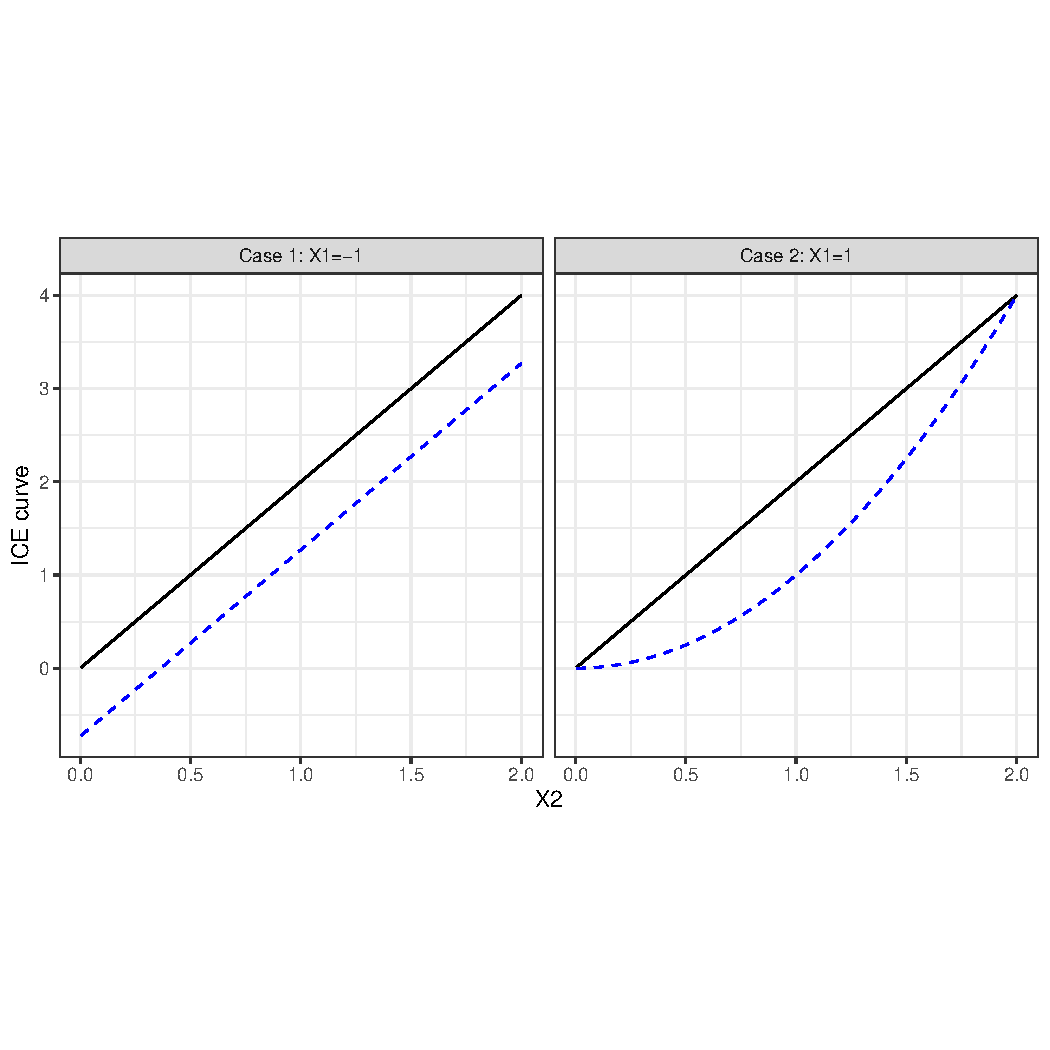
\includegraphics[height=4cm,  width=1\linewidth]{figures/fig-toyexample.pdf}
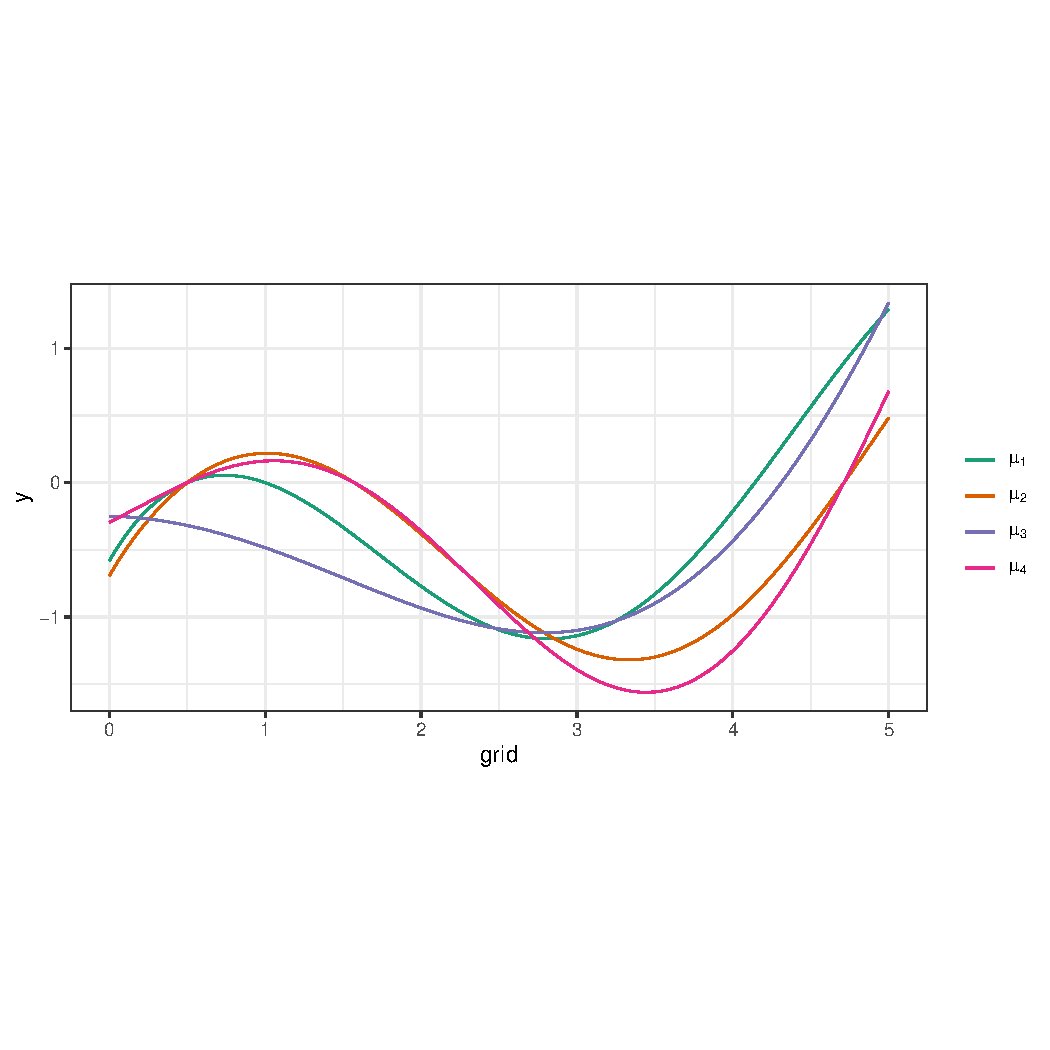
\includegraphics[trim=0cm 4cm 0cm 3cm, clip, scale=.6]{figures/fig-simstudy1.pdf}
\caption{True mean functions. \label{meanfun} }
\end{figure}

Functional data are simulated with a four-cluster structure, based on four functions that represent the mean of each group. Figure \ref{meanfun} shows the true mean functions, $\mu_g(x), \; x \in \left[0, 5\right]$, where $g=1,2,3,4$ indicates the cluster. According to \cite{hitchcock2007effect}, the $\mu_g(\cdot)$ \textit{`... were intentionally chosen to be similar enough to provide a good test for the clustering methods that attempted to group the curves into the correct clustering structure, yet different enough that they represented four clearly distinct
processes.'}

Synthetic data are obtained by adding random noise to $\mu_g(x)$:  
\[ y_{ig} = \mu_g(x_i) + u_g + \epsilon_{ig}, \]
where $u_g \sim N(0, 1)$ and $\epsilon_{ig} \sim N(0, 0.1^2)$. Figure \ref{dataset} shows a simulated dataset, consisting of $N=40$ curves (10 curves from each group) represented in a discretised form, with $n=50$ values per curve, equally spaced in $\left[0, 5\right]$.  

\begin{figure}[hbpt]
\centering
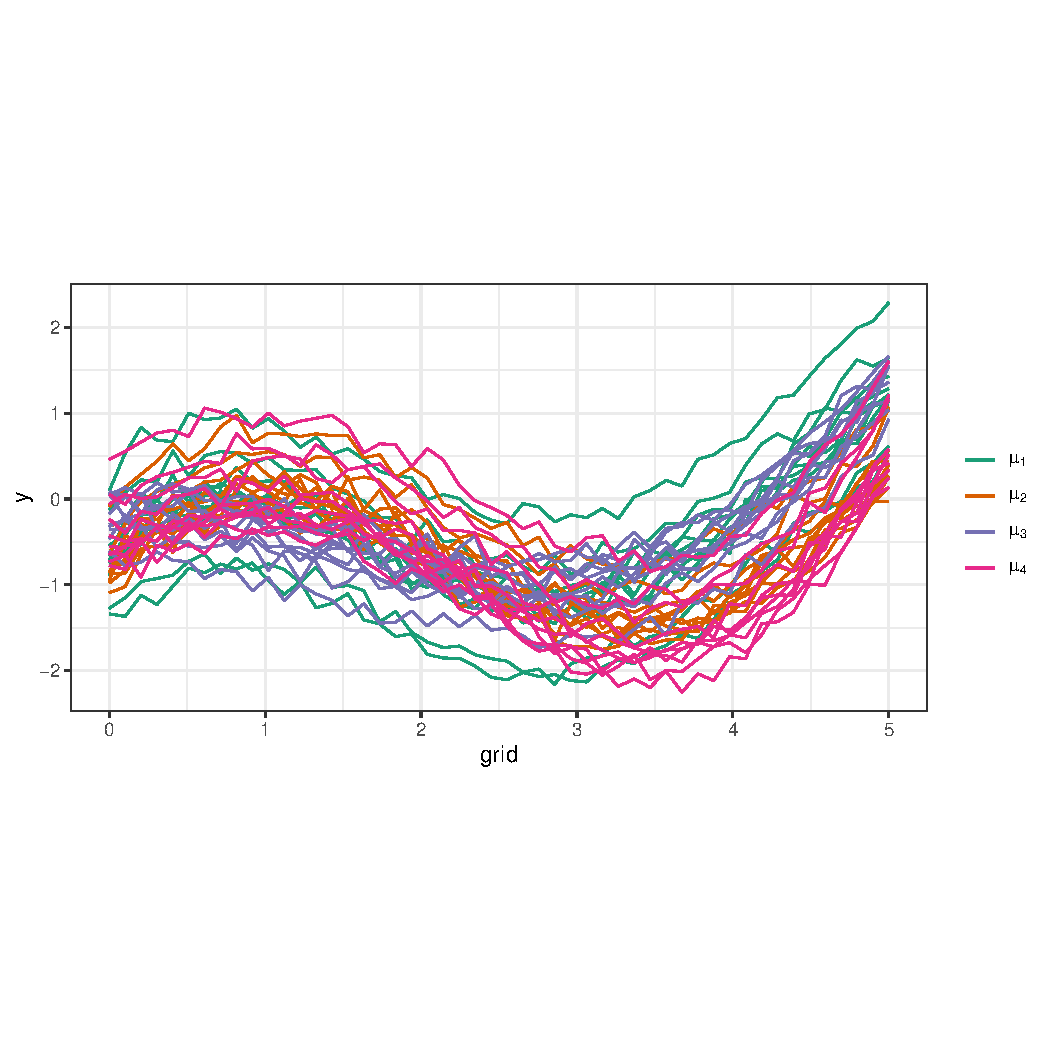
\includegraphics[trim=0cm 4cm 0cm 3cm, clip, scale=.6]{figures/fig-simstudy2.pdf}
\caption{ A simulated dataset. \label{dataset} }
\end{figure} 

The clusters are estimated using the k-medoids method with the \texttt{pam()} function in \texttt{R}, with pre-smoothed data as the main input. Two cluster solutions are obtained for each simulated dataset, 
using the L2 and Sobolev distances as the dissimilarity function. The cluster solution performance is evaluated based on the proportion of pairs of curves that are correctly matched in the same group. The process is replicated $500$ times. 

Table \ref{sim-results} presents results from the 500 replications. Using the Sobolev distance provides a larger proportion of correctly matched pairs on average; additionally, the 5\% quantile of the ratio is slightly larger than 1, so the Sobolev distance resulted in a better performance for at least 95\% of the simulations. 

\begin{table}[ht]
\centering
\caption{Summary of results} 
\label{sim-results}
\begin{tabular}{rrrrr}
  \hline
 & mean & sd & Q0.05 & Q0.95 \\ 
  \hline
L2 & 0.48 & 0.06 & 0.37 & 0.58 \\ 
  Sob & 0.59 & 0.09 & 0.47 & 0.74 \\ 
  Ratio & 1.26 & 0.20 & 1.01 & 1.63 \\ 
   \hline
\end{tabular}
\end{table}


\section{Supplementary figures}
\label{app:figsup}

\begin{figure}[hbpt]
    \centering
    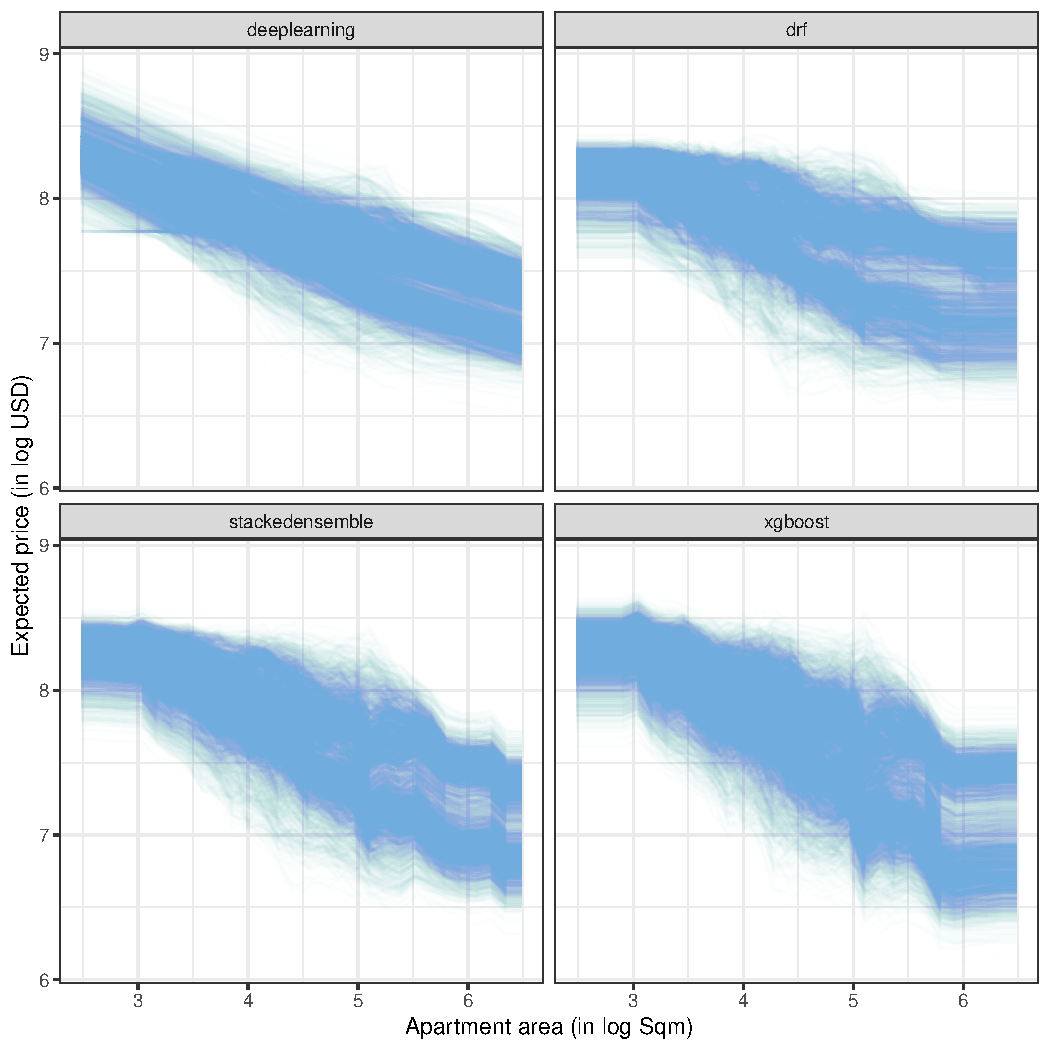
\includegraphics[scale=0.6]{figures/fig-ice-sup-dec.pdf}
    \caption{ICE-plot for the \textit{log apartment area} variable. Each panel corresponds to a predictive model. Five thousand randomly stratified selected curves are shown.}
    \label{fig-icesup}
\end{figure}

\begin{figure}[hbpt] 
    \centering
    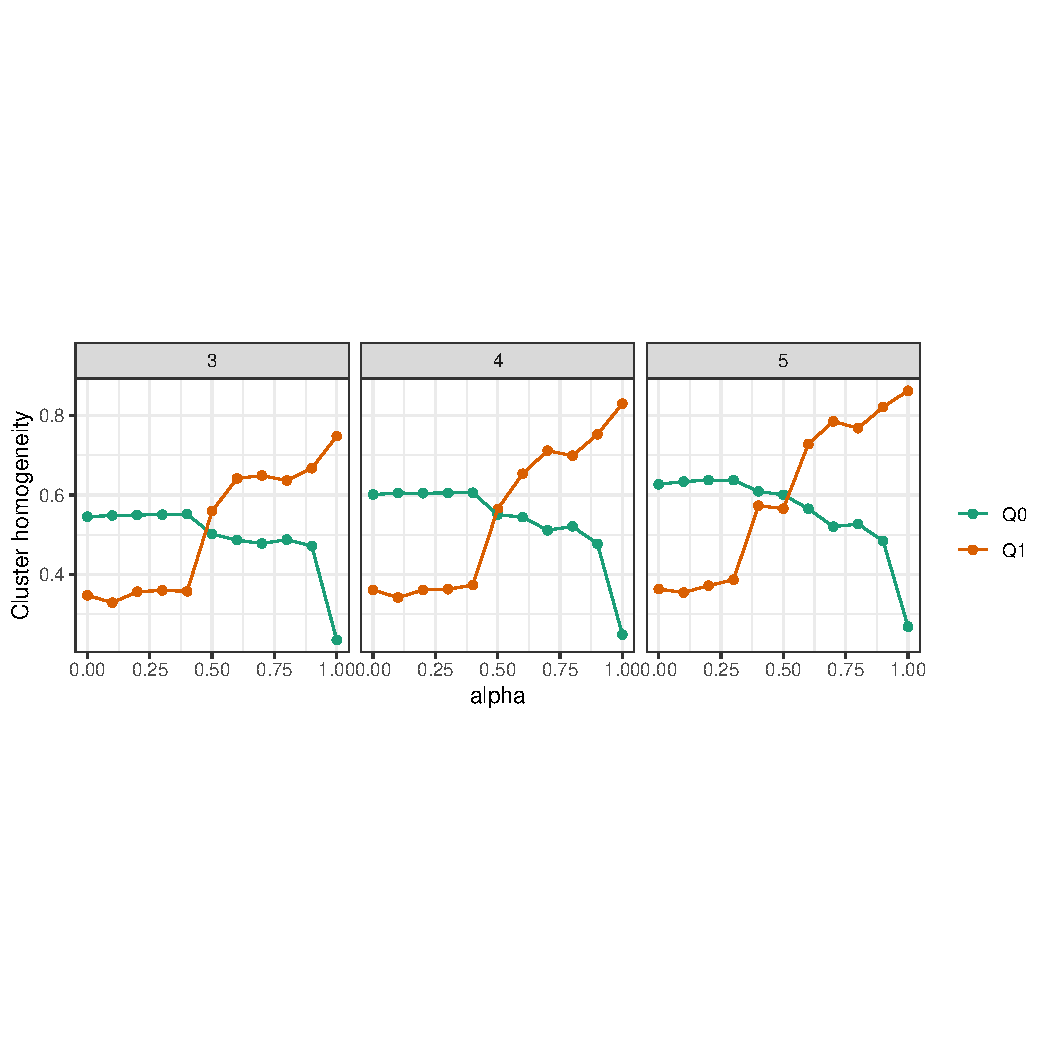
\includegraphics[trim=0 4cm 0 4cm, clip, scale=.6]{figures/fig-alphaoptimo.pdf}
    \caption{Optimal $\alpha$ for different groups.}
    \label{alpfaoptimo}
\end{figure}


\end{document}


% \section{ICE curves in spatial problems} \label{section:2}
% Consider a supervised problem where the objective of statistical learning models is to approximate 
% \[
% \mathbb{E}(Y|X=x) = f(x) \approx \hat f(x);
% \]
% where $X=(X_1,X_2,\dots, X_q)$ is a vector of $q$-variables, $Y$ is the response variable and $\hat f$ is the fitted model that predicts the scalar $Y$ as a function of $X$. In this context, a goal of interpretable methods is to characterize the dependence of the ``main effects'' on $f(x)$ in each explanatory variable. It is also possible to analyze the ``low order'' dependence between pairs of variables. 
% 
% Lets assume the main goal is to understand the effect of a set of explanatory variables denoted as $X_S$ on the response variable in a model agnostic way ($S \in \{1,2,\dots,q\}$ and denote the subset $C$ as the complement of $S$). One of the earliest methods for this is partial dependence plot \citep{friedman2001}. The PD-plot describes the change of the response variable in a model as a function of the marginal effect of one or more variables (subset $X_S$) when averaging the effects of the other explanatory variables (complement subset $X_C$). 
% 
% Main advantages of PD-plot is that its estimation is very intuitive and presents a causal interpretation in the results of any learning model. The main drawbacks are that hide heterogeneous effects, it might be rely on unrealistic set of observations and is computationally expensive. Alternatives to PD-plot has being proposed to overcome its problems, such as accumulated local effects (ALE-plot) \citep{apley2020visualizing} and the individual conditional expectation (ICE-plot) \citep{goldstein2015peeking}.
% 
% \subsection{Individual conditional expectation (ICE-plot)} \label{sub:ICE}
% 
% The ICE-plot is proposed as an extension of PD-plot, to visualize the dependence of the prediction on a feature for each sample separately, with one curve per observation. The method attempts to capture the dependency of the response variable on a set of variables, allowing heterogeneous effects.
% 
% For each observation, the curve $\hat f_{S,ICE}^{(i)}(x_S)$ is obtained by varying $x_S$ in the function $\hat f(x_S,x_C^{(i)})$ while the variables $x_C^{(i)}$ remain constant. That is to say
% \[
%  \hat f_{S,ICE}^{(i)}(x_S)= \hat f(x_S, x_C^{(i)}). 
% \]
% 
% It is worth noting that averaging the ICE curves corresponds the definition of the PD-plot
% \[
% \hat f_{S,PD}(x_S) = \frac{1}{N}\sum_{i = 1}^ N \hat f(x_s, x_C^{(i)});
% \]
% then is possible to interpret the ICE curves similarly as the classic PD-plot but allowing to pick interactions when visualizing the $N$ plots (something that vanish when all ICE are averaged into one curve).
% 
% One disadvantage of ICE plots is the overplotting when big data set are involved. In such cases, it can be challenging to discern any meaningful information due to the overlapping of data points. This is specially relevant for ICE curves since its main purpose is to look for heterogeneity patterns in the predictor effect. Usual graphical solutions such as transparency or 2-dimensional histograms are not suited for plotting lines.  Specifically for ICE-curves, \texttt{h2o} implementation (\cite{hall2017}) choose ICE-curves for decile values (in the observed response), so no matter how large is the sample data, only ten ICE curves are displayed, resulting in an oversimplified plot. An alternative is to plot a stratified sample of curves. This method can be combined with line transparency to allow to reduce the overplotting while is possible to see different patterns of ICE curves in the data. An application of this plot can be found in Figure \ref{fig-icesup} in  Section \ref{section:4}. 
% 
% 
% \subsection{ Spatial ICE curves (SpICE)} 
% \label{seccD}
% Spatial data is any type of data which references a specific geographical area or location. Each curve in the ICE-plot is associated with a specific observation, so it can be link to a geographical location in spatial applications. Combining ICE-plot and spatial structure of the data is possible to overcome some drawbacks of ICE curves and improve interpretability at the same time. 
% In this paper,  SpICE  refers to clustering ICE curves with spatial contiguity constrains. 
% 
% 
% The Ward-like method is used for the construction of the clusters, see \cite{chavent2018}. This is based on two dissimilarity matrices ($D_0$ and $D_1$) and a mixing parameter $\alpha \in [0,1]$. $D_0$ is a dissimilarity matrix between ICE curves and $D_1$ is a dissimilarity matrix that consider the spatial problem.
% 
% Matrix $D_0$ is determined only based on a dissimilarity measure between each ICE curve. The key idea is to group together observations with similar predictor effect on the response that could be summarize as the level and change range of the ICE curve. For this reasons it is appropriate to consider a distance  that not only considers the value of the integral but also their growth/decrease. However, some ICE curves might not be differentiable in some point for a lot of statistical learning models. One way to overcome this issue and obtain estimates in a $C^1$ space, is to consider the curve $\widetilde{f}_{S,ICE}^{(i)}(x_S)$ that is the convolution of the function  $\hat{f}(x_S, x_C^{(i)})$  with a Gaussian kernel. That is,  
% \begin{equation}\label{convo}
%  \widetilde{f}_{S,ICE}^{(i)}(x_S) := \ \hat{f}(x_S, x_C^{(i)}) \ast K_h(x_S),
% \end{equation}
% where $K_h$ is the Gaussian kernel, $h$ the smoothing parameter and $\ast$ the convolution operation.  For the function $\widetilde{f}_{S,ICE}^{(i)}(x_S)$ in the equation (\ref{convo}) it is possible to use the Sobolev $W^{1,2}(\mathbb{R})$ metric \citep{sobolev},  induced by the norm
% \[
% \Vert  \widetilde{f}_{S,ICE}^{(i)}(x_S)   \Vert= \sqrt {\int \vert  \widetilde{f}_{S,ICE}^{(i)}(x_S)  \vert ^2 dt + \int \vert  \widetilde{f}_{S,ICE}^{\ '(i)}(x_S) (t) \vert ^2 dt}.
% \]
% Assuming the true $f(x)$ is a smooth function, the above transformation of ICE curve (the convolution) will not distort the ICE estimator in a relevant way. 
% 
% For the definition of the distance $D_1$  is necessary use the spatial information associated with each observation. Depending on the quality and nature of the spatial data available (such as coordinates points, or area data, etc) this metric distance could be defined in different ways. In the motivating example of this paper %with the data described in Section \ref{section:3}, 
% the Euclidean distance between coordinates observations is used for simplicity.   
% 
% Let us consider a partition $\mathcal{P}_K = (C_1 ,\ldots , C_K )$ in $K$ clusters of ICE curves. Clustering algorithm proposed in \cite{chavent2018} is outlined in order to described how to choose a value for mixing parameter. First, consider $n$ observations, where $w_i$ represents the weight associated with the $i$-th observation. Let $D_0=[d_{0,ij}]$ and $D_1=[d_{1,ij}]$ be two dissimilarity matrices of size $n \times n$, associated with the $n$ observations, corresponding to the covariates and spatial constraints, respectively. Both dissimilarities are normalized to make them comparable. The pseudo-inertia of a group is now also indexed by the mixing parameter $\alpha$, which weighs the importance of the two dissimilarities. The mixed pseudo-inertia of the $k$-th group is defined as
% 
% $$I_{\alpha} \left( C^{\alpha} _k \right)=  (1-\alpha) \sum_{i \in C^{\alpha}_k} \sum_{j \in C^{\alpha}_k} \frac{w_i w_j}{2 \mu^{\alpha}_k}d^2_{0,ij}+\alpha \sum_{i \in C^{\alpha}_k} \sum_{j \in C^{\alpha}_k} \frac{w_i w_j}{2 \mu^{\alpha}_k}d^2_{1,ij};$$
% with $\mu^{\alpha}k= \sum{i \in C^{\alpha}_k} w_i$, and the inertia of the partition with $K$ groups is given by
% $$W _{\alpha}\left( \mathcal{P}^{\alpha}_{K} \right)= \sum_{k=1}^K I_{\alpha} \left( C^{\alpha}_k \right).$$
% Secondly, given a partition into $K+1$ groups, now the Ward type algorithm is applied to obtain a new partition into $K$ groups, which is a solution to the following optimization problem,
% $$\textrm{arg}  \min\limits_{A,B \in \mathcal{P}_{K+1}^{\alpha}}\, I_{\alpha}\left( A \cup B\right) - I_{\alpha}\left( A \right) - 
% I_{\alpha}\left(B \right) .$$
% Finally, a criteria are developed for choosing the mixing parameter $\alpha$ is based on the notion of the proportion of total mixed pseudo-inertia explained by the partition $\mathcal{P}_K^{\alpha}$ into $K$ groups,
% $$Q_{\beta}( \mathcal{P}_K^{\alpha})= 1- \frac{W_{\beta} \left( \mathcal{P}_{K}^{\alpha} \right)}{W_{\beta}\left( \mathcal{P}_{1} \right)} \in [0,1]\,; \:\: \text{ with } \beta \in [0,1] \,,$$
% where $W_{\beta}\left( \mathcal{P}_{1}\right)$ represents the total pseudo-inertia based on the dissimilarity matrix $D_0$ if $\beta=0$, the total pseudo-inertia based on the dissimilarity matrix $D_1$ if $\beta=1$, and if $\beta \in (0,1)$ it is the total mixed pseudo-inertia
% 
% The parameter $\alpha$ regulates the two factor's weight  involved in the algorithm. On the one hand, when $\alpha=0$ the clusters are just determined by covariates without spatial information and on the other hand when $\alpha=1$ the clusters are just determined by the spatial information. Ideally is desirable to determine $\alpha$ value which increases cluster's spatial continuity without loosing cluster homogeneity in terms of ICE curves.
% 
% \section{Application results}
% \label{section:3}
% %In this Section data description, predictive models with `h2o` and SpICE curves results are presented.
% This Section start by describing the dataset used as motivating example, then performance results of statistical learning models and interpretable methods are presented. Finally, the SpICE curves results in the motivating example data are presented. 
% 
% \subsection{ Dataset: Appartment prices in Montevideo }
% The data in this paper are from an eCommerce platform \href{https://www.mercadolibre.com.uy)}{Mercado Libre} where real estate are offered for sale and rental. The complete data set contains asking price information for properties in Montevideo, capital city of Uruguay from February 2018 to January 2019 \citep{Picardo}. There are 92,832 observations and 116 variables in the complete data set. Nevertheless, only apartments data will be consider for the analysis working with 70,817 apartment observations for sale in Montevideo.
% 
%  Figure \ref{mapa} shows the distribution of asking prices for apartments in Montevideo. Each dot on the plot represents one apartment available for sale, while the color of the dot indicates the asking price per square meter in US dollars.
% Figure \ref{mapa} suggest locations close to the coast are associated with higher price range. Apartment's asking price ranges from  541 to 5000 US-dollars per square meters in Montevideo and the median value is close to 2500 US-dollars. 
%  \begin{figure}[hbpt]
% \centering
% 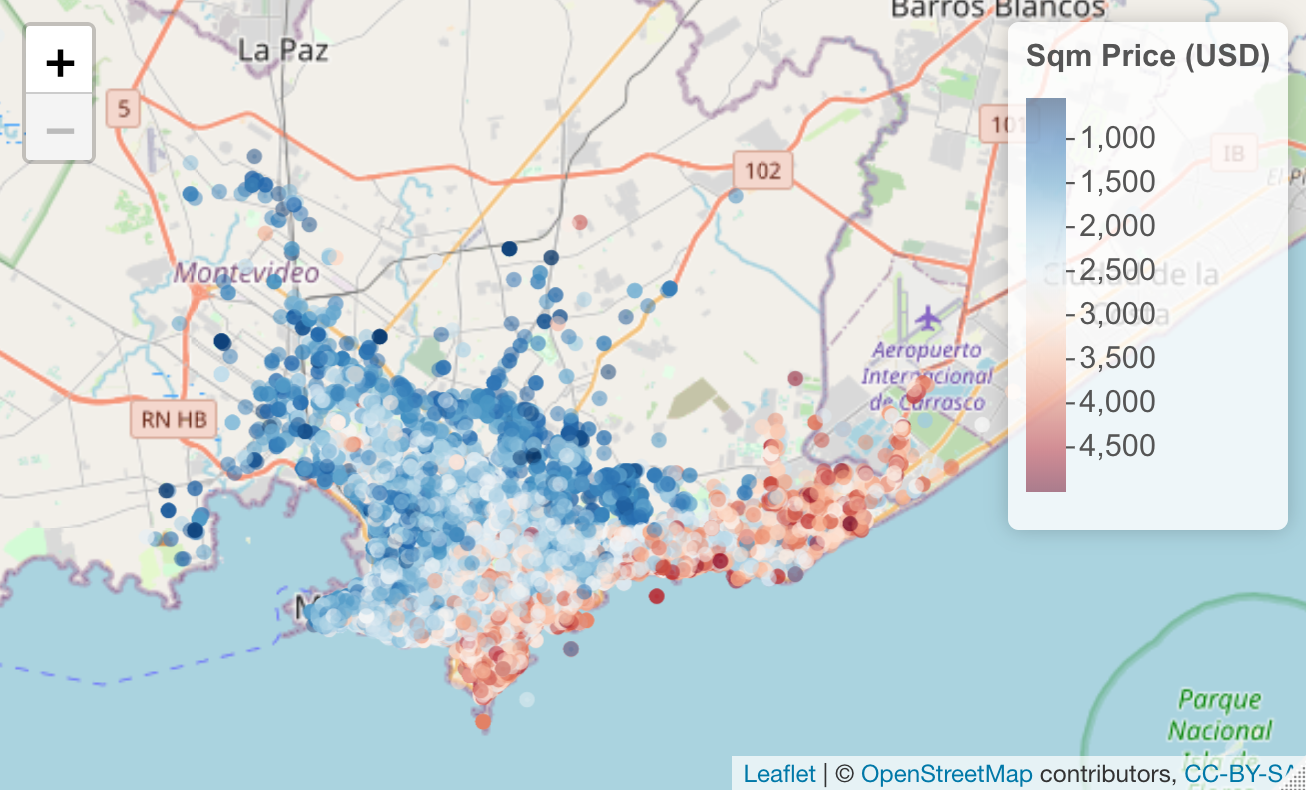
\includegraphics[width=1\linewidth]{figures/mapa_preciom2.png}
% \caption{Distribution of asking price apartments in Montevideo. Each dot represents one apartment and the color is the asking price per square meter in US dollars. 
% \label{mapa} }
% \end{figure}
% 
% \begin{table}[hbpt]
% 	\centering
% 	\caption{Variable description\label{tabvar} }
% \scriptsize
% \begin{tabular}{p{2.4cm}p{2.4cm}p{7cm}}
% 		\hline \\[-1.8ex] 
% \textbf{Variable} & \textbf{Role} &  	\textbf{Description} \\
% 		\hline \\[-1.8ex] 	\hline \\[-1.8ex] 
% 
% \texttt{lpreciom2} & Response & Log of asking price in US-dollars per square meters. \\ \hline
%   
% \texttt{amenities} & Explanatory & Total number of amenities presented in the apartment.\\
% \texttt{bedrooms} & Explanatory & Bedrooms quantity. Reduced to values between 0 (studio) and 3. \\
% \texttt{bathroom} & Explanatory & Bathrooms quantity. Reduced to values between 1 and 3.\\
% \texttt{elevators} & Explanatory & Elevators quantity. Reduced to values between 0 and 2. \\
% \texttt{condition} & Explanatory & Property condition (new/used).  Properties with less than 1 year were marked as ``new''.\\
% \texttt{expenses} & Explanatory &  Numerical value representing monthly expenses in Uruguayan pesos (local currency)\\
% \texttt{garage} & Explanatory & Whether or not there is a garage. Reduced to values between 0 (``No'') and 1 (``Si'').\\ 
% \texttt{ldistance\_beach} & Explanatory & Minimum distance (Euclidean)  between  the property   and the beach (in log scale). \\
% \texttt{lsup\_constru} & Explanatory & Log of  area in square meters. Values over 2000  or under 9 square meter were remove from data. \\
% \texttt{neighborhoodgr} & Explanatory &  Montevideo neighborhoods grouped by proximity in 12 regions. \\ \hline
% \texttt{lat} & Spatial & Property latitude coordinate \\
% \texttt{long} & Spatial & Property longitude coordinate \\
% 	\hline \\[-1.8ex] 	\hline \\[-1.8ex]  
% 	\end{tabular}
% \end{table}
% Table \ref{tabvar} presents the selected variables from the entire dataset to use for the statistical methods applied latter, indicating variable name in the dataset, its role in the statistical analysis and a brief description. All the models are fitted using as response variable the natural logarithm of the  price per square meters (\texttt{lprecio2}). The explanatory variables represent apartment features commonly used in real estate modeling, such as location (\texttt{neighborhoodgr}), total area, number of bedrooms and number of bathrooms. In addition, with the available information we create additional explanatory variables such as distance to the beach and total amenities. A reduced number of variables were selected to assure data quality from the complete data set. Finally, geographical coordinates of each property are used as additional information to improve interpretability using SpICE curves described earlier.
% 
% \subsection{Predictive models with \texttt{h2o} }
% \label{modelo} 
% 
% Several models were trained %to estimate $f(x_i)$ 
% using the automatic machine learning (\texttt{autoML}) procedure from \texttt{h2o} R package \citep{h2o} to predict the apartment  price as an alternative to classical methods. The  \texttt{autoML}  estimates models well tuned in 4 families: penalized linear models (glm), random forest (drf), xgboost, and Deep Learning. In the rest of the paper, the best model of each family and an additional metalearner are used. 
% 
% Table \ref{comparo} shows the  performance measures for the selected predictive models. The root mean square error (RMSE) and the $R^2$ are used to evaluate model performance. These values are computed with the response variable in logs (as it was used for trained every model). Additionally, mean absolute error (MAEo) and mean absolute percentage error (MAPEo) are both computed in the original scale of the response variable so can be read in dollars per square meter.  The four measures are computed using a testing data set different from training sample (2/3 training and 1/3 testing). 
% 
% \begin{table}[ht]
\centering
\caption{Predictive performance measures by model} 
\label{comparo}
\begin{tabular}{rlrrrr}
  \hline
 & model & rMSE & R2 & MAEo & MAPEo \\ 
  \hline
1 & stackedensemble & 0.14 & 0.81 & 242.68 & 9.58 \\ 
  2 & drf & 0.14 & 0.80 & 251.08 & 9.94 \\ 
  3 & xgboost & 0.15 & 0.80 & 254.48 & 10.06 \\ 
  4 & deeplearning & 0.20 & 0.63 & 395.84 & 15.18 \\ 
  5 & glm & 0.22 & 0.55 & 427.72 & 17.13 \\ 
   \hline
\end{tabular}
\end{table}

% 
% In terms of predictive performance, stacked metalearner, Random Forest and the XGboost algorithms show similar performance, somewhat better than the deep learning method or the penalized linear model. It is worth to note the stacked model combines 7 tree based models in its construction. On average, the best model get an average error in the asking price of \$245 per square meter, around 10\% of the observed price.  %The variability explained by  every model is between $0.74$ and $0.90$. 
% 
% \subsection{ Variable importance measures}
% \label{4.2} 
% The first approach to interpreting model results for statistical learning methods is to compute variable importance measures. Importance variable measures are  widely used for this problem. Some variable importance  measures are model specific but other are model agnostic and can be computed for any model. Explanatory variables with bigger values in this measure indicate that are more important for the predictive model and have more impact on the response variable. However, the weakness of this method is that has no information about the effect direction or shape.
% 
% Variable importance measures were computed for each model. The measures were scaled so that the most important variable in each model has a value of 1, which simplifies the model comparison. 
% Figure \ref{fig-imp} shows the results  by model for the variable importance. The predictors ordering are similar in all models.  The apartment area (\texttt{lsup\_constru}) and the neighborhood (\texttt{neighborhoodgr}) are the two most important variables to predict the apartment price. All the tree based methods (drf, xgboost and stackedemsemble) shows a third relevant variable which is the distance from the apartment to the beach (\texttt{ldistance\_beach}). The rest of the predictor variables are not relevant for prediction. 
% 
% \begin{figure}[htpb]
%     \centering
%     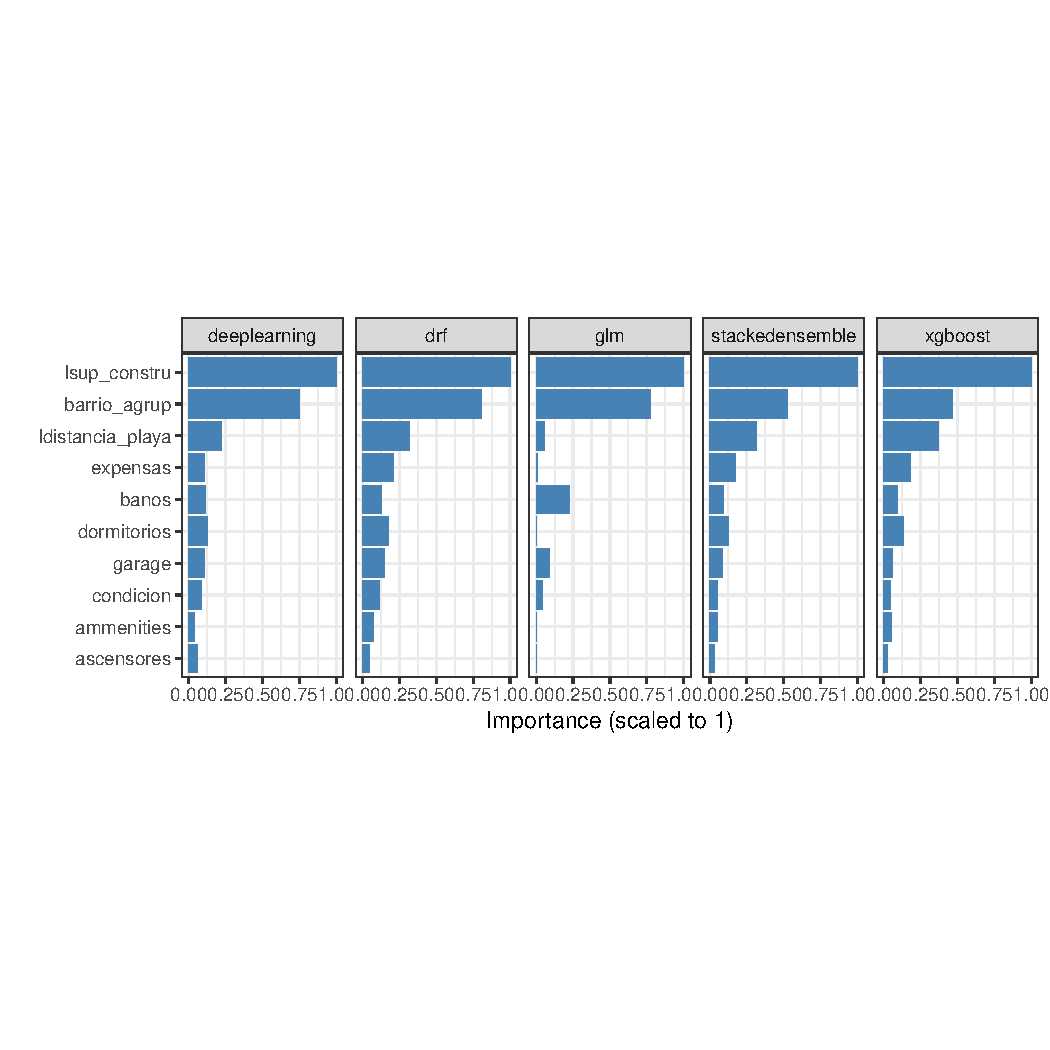
\includegraphics[trim=0cm 4cm 0cm 4cm, clip, scale=1]{figures/fig-importance.pdf}
%     \caption{Variable Importance. Each panel represents a model, and the y-axis shows the variables included in all the models. Bar length represents the scaled variable importance measure to predict the apartment price.}
%     \label{fig-imp}
% \end{figure}
% 
% \subsection{ Partial effect of apartment area } \label{sub:resultados_pdp}
% Variable importance measure gives a ranking  of variables according to their relevance to predict the response variable.  However, they do not provide information on the effect that the individual variables have on the response. In order to characterize the average effect of apartment features on its  price, the PD-plot and the ALE-plot  are estimated. The algorithms used for its estimation  were done using R packages \texttt{pdp} \citep{pdp} and \texttt{ALEPlot} \citep{aleplot}. 
% %interpretable methods described in Section \ref{section:2} are computed. Computations of the PD-plot, ALE-plot and ICE curves are done using R packages \texttt{iml} \citep{iml} and \texttt{ALEPlot} \citep{aleplot}. 
% \begin{figure}[hbpt]
%     \centering
%     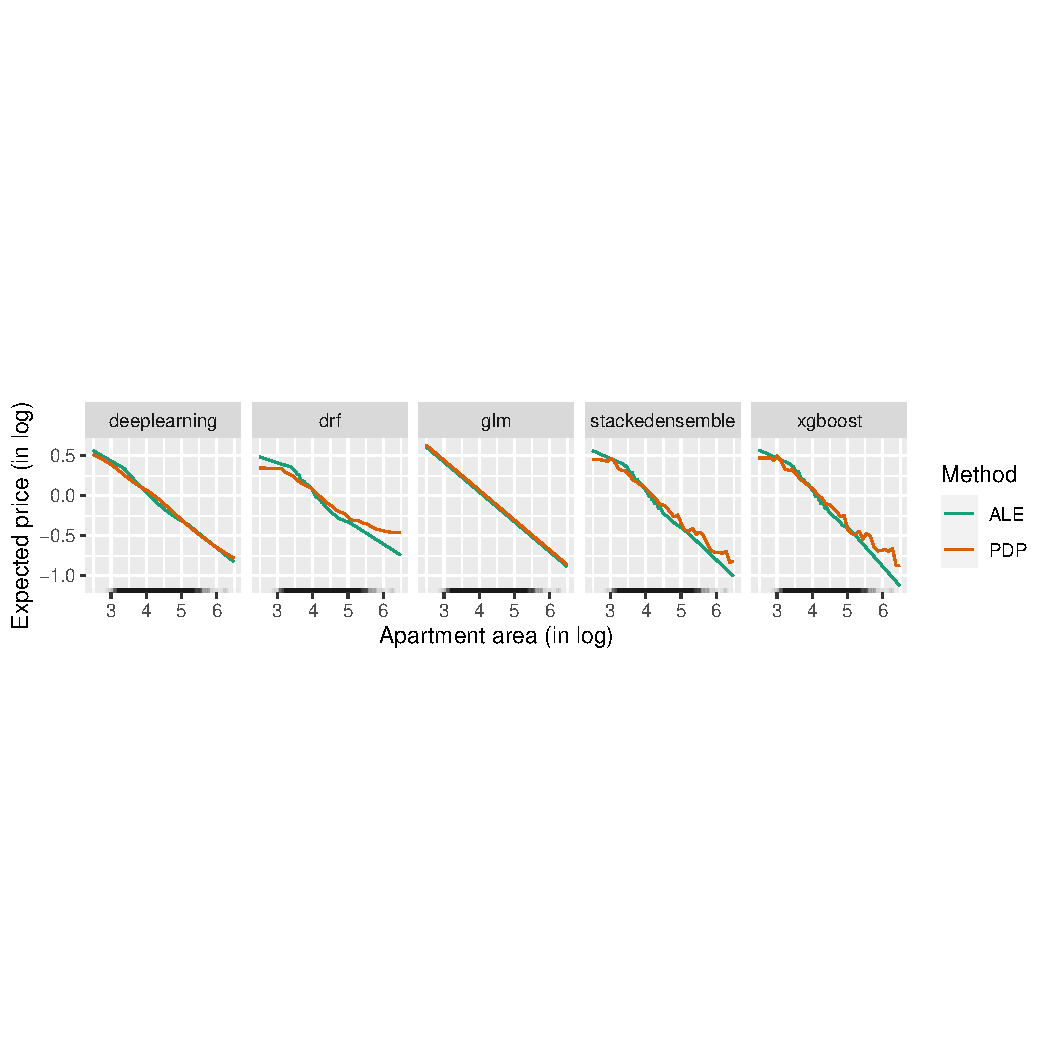
\includegraphics[trim=0cm 6cm 0cm 6cm, clip, scale=1]{figures/fig-efecto-lsub.pdf}
%     \caption{Effect of \texttt{lsup\_constru} variable in different models. Each panel corresponds to a predictive model and color represents the interpretable method (ALE-plot or PD-plot).}
%     \label{fig-pdpalesup}
% \end{figure}
% 
% Apartment area (\texttt{lsup\_constru}) is the most relevant feature in every model. The effect of this variable on the response is described with PD-plots and ALE-plots shown in Figure \ref{fig-pdpalesup} where each panel corresponds to a specific model. A negative effect is suggested by these plots with similar effect in every model. This is  true especially in the middle of the range for apartment area where there is most of the observed sample. Some differences can be seen in very large or very small apartments where random forest and XGboost show smaller effects on prices. %Estimated results for PD-plot and ALE-plot are very close. This might suggest the correlations among explanatory variables are not too high to bias the estimated effect with PD-plot and then the local correction made by ALE-plot has no effect. 
% 
% Specifically, Figure \ref{fig-pdpalesup} shows the average effects of the variable \texttt{lsup\_constru}  in the sample. In a scenario where the impact of an explanatory variable over the response presents heterogeneity among observations, PD-plot and ALE-plot methods hide the variability of effects. An alternative method for interpretability to tackle this issue is the ICE-plot. The value of visualizing the individual curves that compose the PD-plot, is to explore other patterns in the effects than just the mean value.  Figure \ref{fig-icesupRF} shows the individual conditional expectation plot for  apartment area (\texttt{lsup\_constru}) for the  random forest model. The other predictive models shows similar results, as can be seen in Figure \ref{fig-icesup} in the Appendix. As it mentioned in Section \ref{section:2} there are too many ICE curves to display, using only transparency it was not enough to produce a good plot. ICE curves of a random sample using observed response deciles as strata are shown. 
% 
% \begin{figure} 
%     \centering
%     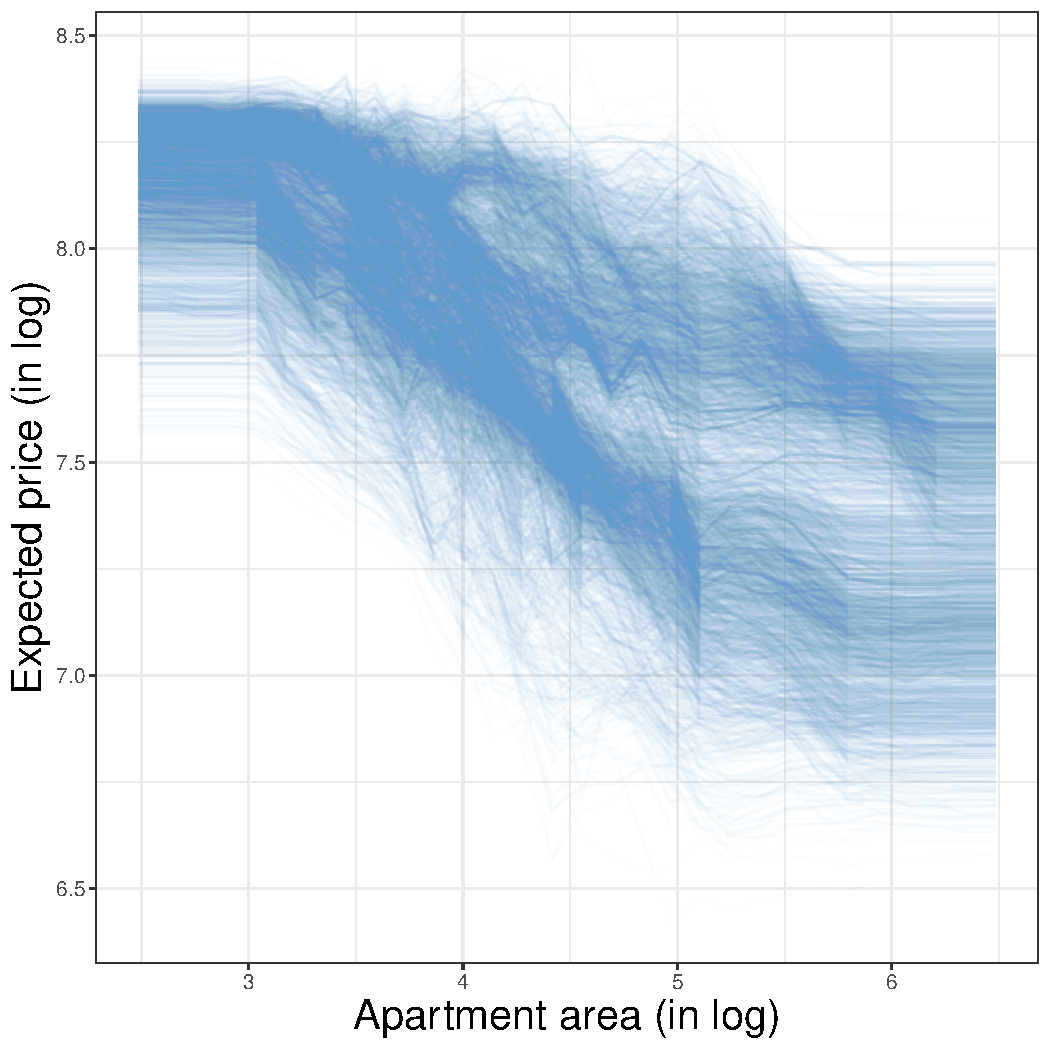
\includegraphics[scale=0.5]{figures/fig-ice-sup-decRF.pdf}
%     \caption{ICE-plot for \texttt{lsup\_constru} variable. Each panel corresponds to a predictive model. Showing 5000 randomly stratified selected curves.}
%     \label{fig-icesupRF}
% \end{figure}
% 
% The results illustrate the negative effect of the variable \texttt{lsup\_constru} in each individual curve. However, it is relevant to note that the effect  present  heterogeneity in the different properties. Figure \ref{fig-icesupRF} suggests that properties with higher predicted prices exhibit a small and linear effect, whereas cheaper properties show a non-linear relationship, with a larger impact of the apartment area.
% 
% \subsection{ SpICE curve effects } \label{results-ice}
% Finally, to explore the connection among ICE curves and geographical location of properties, SpICE curves results are presented.  
% 
% In order to compute $D_1$ matrix (see Section \ref{seccD}), Euclidean distance between apartment coordinates is used. 
% This metric is easy to visualize and applicable in the city of Montevideo due to the relatively close distances involved (maximum 30 km). However, it is possible to define other metrics using these two variables or other variables that better characterize the distance between two properties.
% 
% The range of the number of clusters is defined as three to five clusters. For each value within this range, an optimal value for the $\alpha$ parameter is determined as a compromise between the within-cluster homogeneity in terms of ICE curves and geographical proximity.
% Results are shown in Figure \ref{alpfaoptimo} in the appendix, final choice is to work with four groups and $\alpha = 0.5$. 
% 
% Figure \ref{fig-spice} shows the results of the geographically constrained clusters. Each apartment for sale in Montevideo city is represented as a point on the map, which is connected to an ICE curve in the bottom panel. The colors of the points and curves indicate the corresponding cluster assignments. Cluster location suggest a layout in the NorthWest-SouthEast direction, similar to the price gradient present in the data (see Figure \ref{mapa}). The apartments in the west and north-west side (green cluster) corresponds low income neighborhoods while the East side of the city (red cluster) represents the highest income zone in Montevideo.  
% 
% Focusing on the SpICE curves presented in Figure \ref{fig-spice}, there are distinct patterns in the relationship between apartment area and the asking price per square meter. Across all clusters, there is a negative relationship between the price per square meter and the apartment area. However, the effect of apartment area on square meter price differs between the green and blue clusters (associated with medium and low-income neighborhoods) and the red and violet clusters (associated with high-income neighborhoods). In green and blue clusters, an increase in apartment area results in a larger decrease in price per square meter compared to the red and violet clusters. This suggests that, in high-income neighborhoods, the total apartment price is more sensitive to changes in apartment area than in low-income neighborhoods where the total apartment prices are more inelastic to changes in apartment area. Consequently, the additional square meter in the apartment has no impact on the apartment price, leading to a decline in the square meter price within the low and medium-income neighborhoods.
% 
% 
% \begin{figure} 
%     \centering
%     %{figures/fig-4grupos.pdf}
%     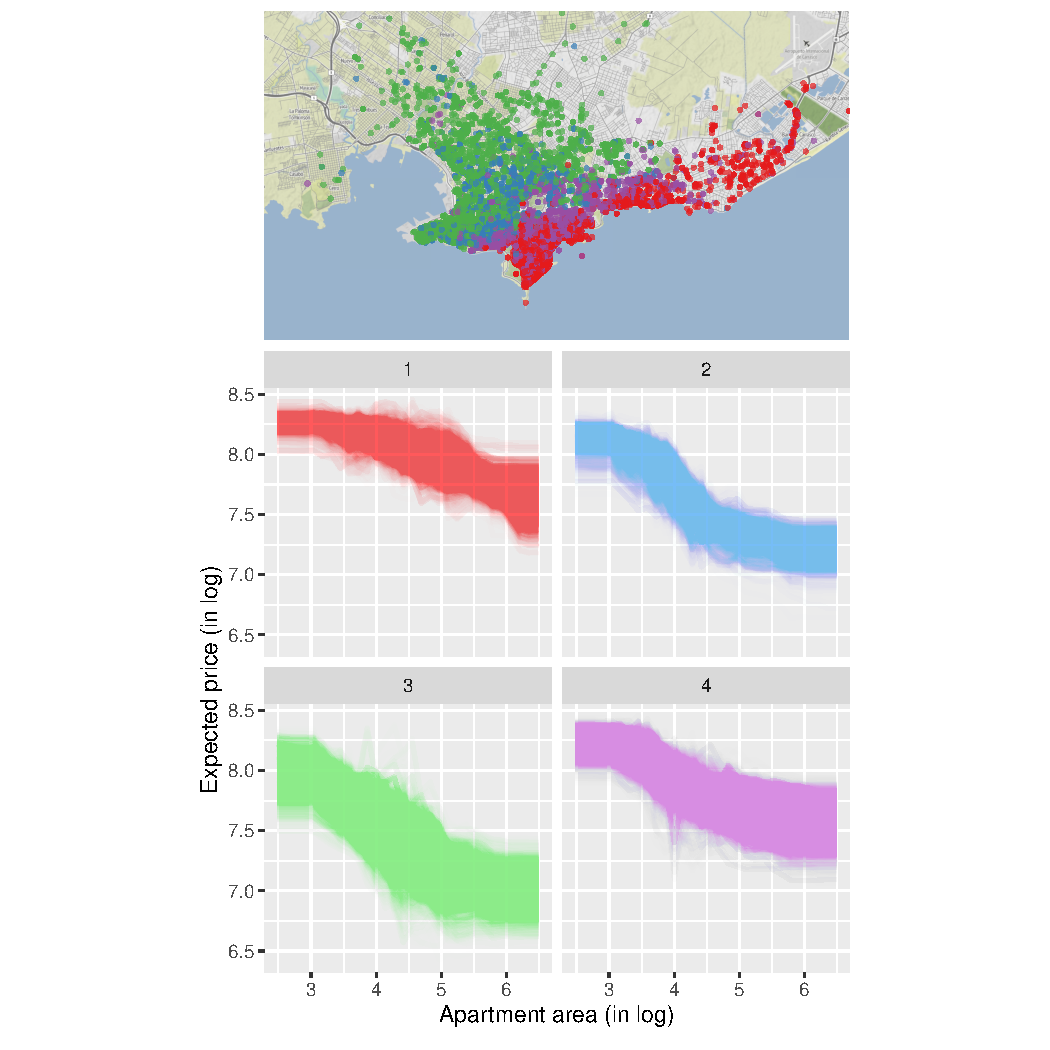
\includegraphics[scale=0.9]{figures/fig-4grupos-alpha5.pdf}
%     \caption{SpICE curves and geographical location of clusters.}
%     \label{fig-spice}
% \end{figure}
% 
% % The properties maps show in the bottom left corner a few apartments located in a low income zone of the city, all points belong to the blue cluster but one which correspond to violet cluster. Figure \ref{fig-spice-zoom} shows SpICE curves for these apartments, as an example to illustrate the reason that geographically close point are classified into different groups. SpICE curve for the violet point show a linear negative effect of the total area, while blue curves of the close by apartments shows a highly non-linear effect of the apartment area. 
% % \begin{figure} 
% %     \centering
% %     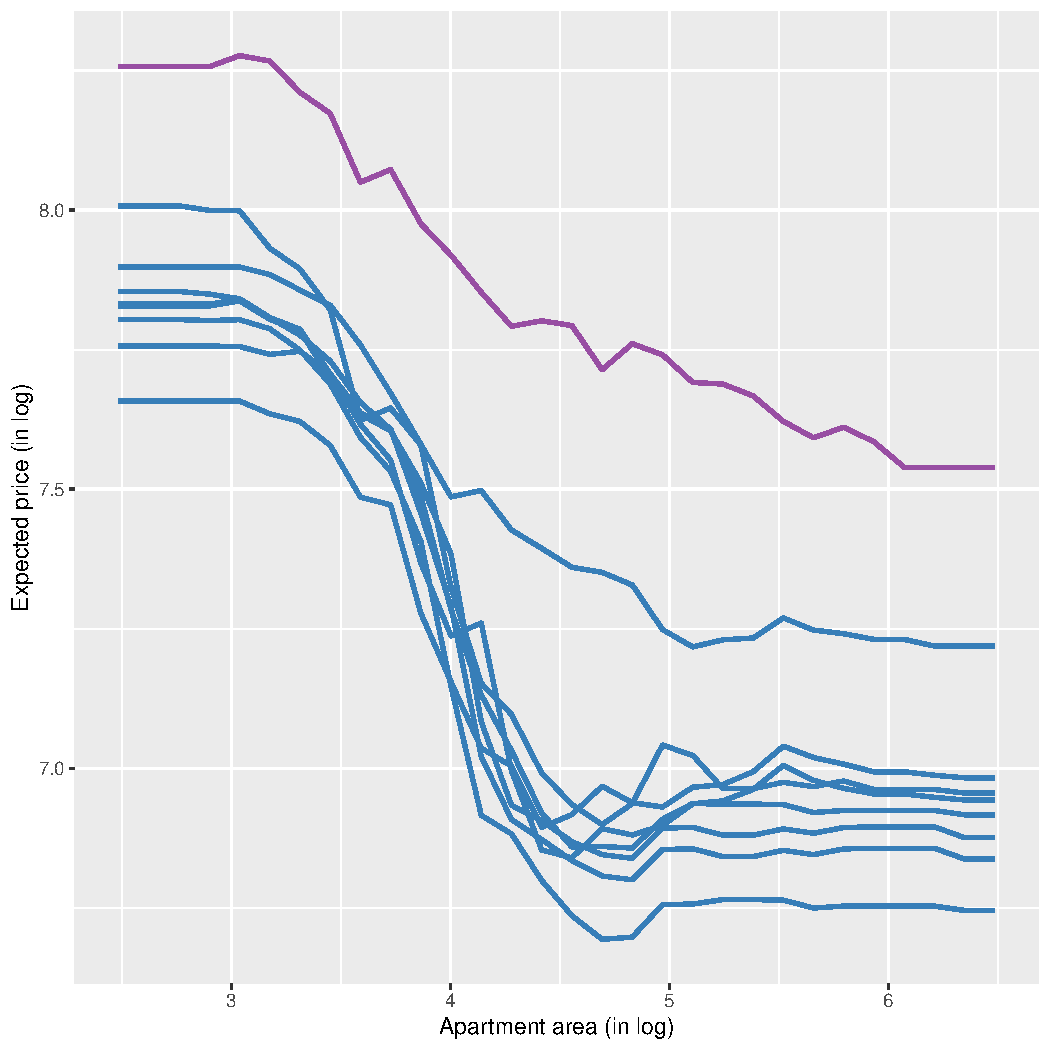
\includegraphics[scale=0.65]{figures/fig-casa-cerro.pdf}
% %     \caption{An example of ICE curves away (blue and violet) from spatially close apartments.}
% %     \label{fig-spice-zoom}
% % \end{figure}
% 
% \newpage
% 
% \section{Discussion} \label{section:4}
% In this paper, model-agnostic interpretable methods for black box models were combined with spatial information to enhance interpretability in spatial applications. Specifically, the paper introduces the concept of geographically constrained clusters of ICE curves, referred to as SpICE curves.
% Similar to ICE plots, SpICE curves can reveal heterogeneous effects of a predictor variable in a black box model.
% The advantage of SpICE curves lies in their ability to interpret multiple clusters simultaneously, making them more suitable for large-scale data applications. Additionally, the spatial contiguity of the clusters provides additional interpretable information, further improving the analysis.
% 
% 
% In the motivating example, SpICE curves were utilized to analyze the impact of the total area of properties on the price per square meter in apartments located in Montevideo city. Five statistical learning methods were chosen from a subset of 25 fitted models, based on their predictive performance using the \texttt{h2o} package with \texttt{autoML} procedure. The apartment's total area emerged as the most relevant feature in all five models, confirming its importance.
% 
%  Then using a fitted model with Random Forest algorithm, ICE-plot and SpICE curves for each apartment were computed. Property spatial information is combined with ICE curves to gain interpretability. Four property clusters were selected, based on a distance that combines a functional distance between ICE curves and Euclidean distance between apartment geographical coordinates.  Clusters blue and green mainly represent properties located in low or mid-low income zones in Montevideo and these clusters present a large, negative, non-linear effect of the apartment area on the price per square meter. On the other hand, clusters violet and red mainly correspond to mid high and high income neigborhoods, showing a small,  close to linear effect of the property area. 
% 
% This paper suggests several aspects that could be explored in future work. Firstly, the improvement of the functional distance used among ICE curves could be considered, such as the utilization of a weighted functional distance, as proposed in \cite{chen2014optimally}.  Secondly, instead of constructing fixed clusters of ICE curves, an alternative approach could involve considering local averages of the ICE curves in a nearest neighbors fashion,  where the distance used to determine the neighbors combines the structure of the ICE curves with geographical distance. Finally, a potential enhancement could involve summarizing the cluster ICE curves using ALE-plots, rather than relying on the average of clustered ICE curves. 
% 
% \section{Supplementary materials}
%  This article was written with the R packages \texttt{knitr} \citep{knitr}, \texttt{ggplot2} \citep{hadley:2016}, \texttt{leaflet} \citep{leaflet}, \texttt{tidyverse} \citep{tidyverse}, \texttt{h2o} \citep{h2o}, \texttt{ClustGeo} \citep{clustGeo},
%  \texttt{KernSmooth} \citep{KernSmooth} and the files to reproduce the article and results is available at https://github.com/natydasilva/SpICE\_COST. 
% 
% \renewcommand{\refname}{References }
% \pagebreak
% \bibliographystyle{chicago}
% \bibliography{bibcsic.bib}
% 
% 
% \appendix
% \section{Supplementary figures}
% 
% \begin{figure} 
%     \centering
%     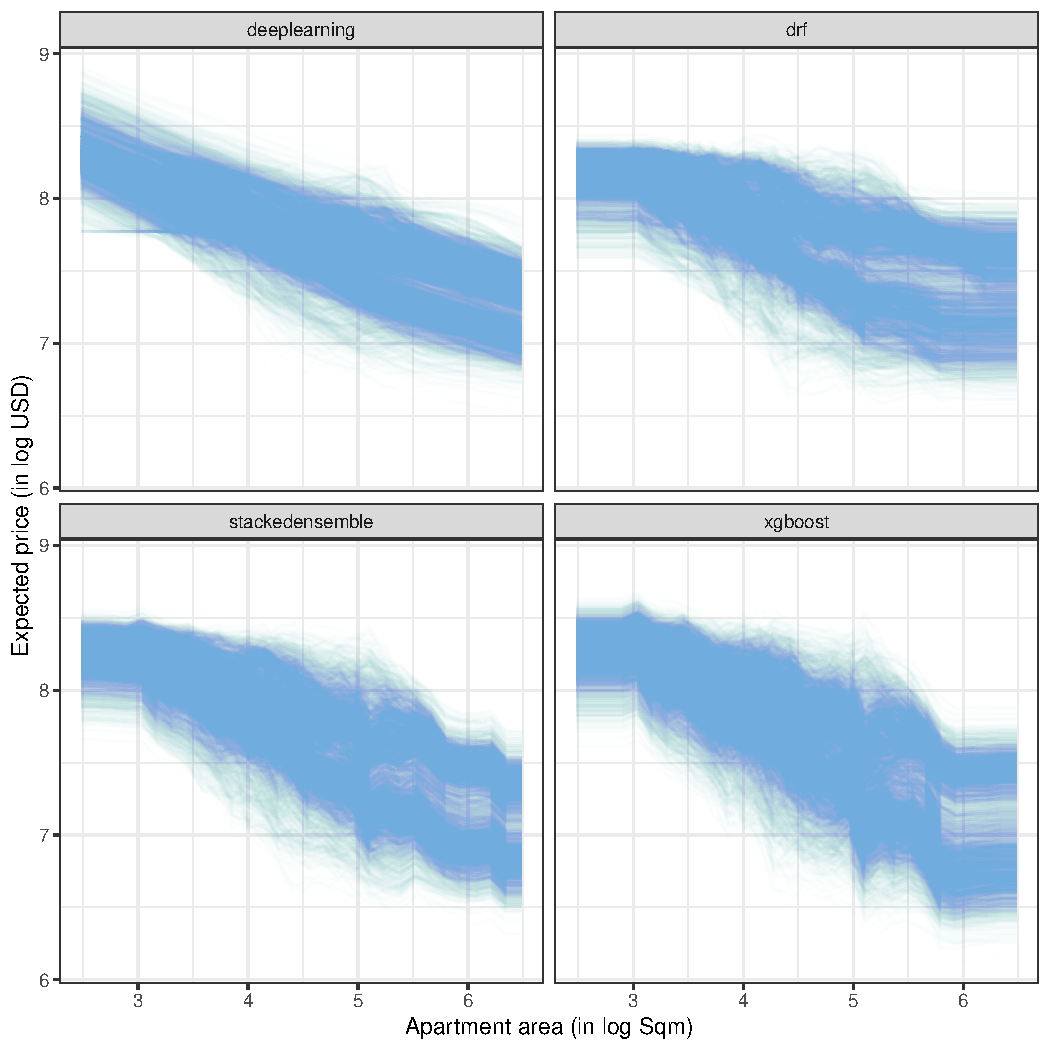
\includegraphics[scale=0.65]{figures/fig-ice-sup-dec.pdf}
%     \caption{ICE-plot for \textit{log apartment area} variable. Each panel corresponds to a predictive model. Showing 5000 randomly stratified selected curves.}
%     \label{fig-icesup}
% \end{figure}
% 
% \begin{figure} 
%     \centering
%     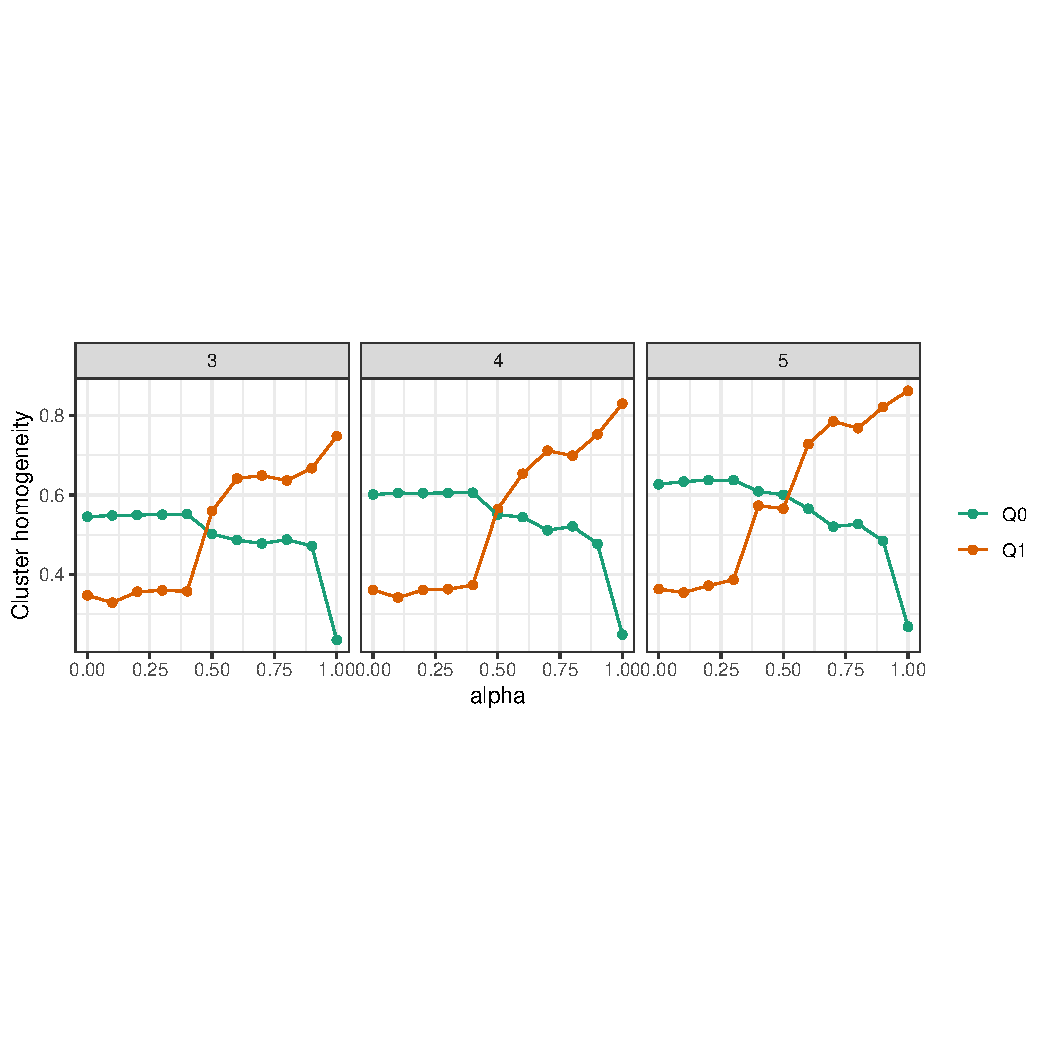
\includegraphics[scale=.6]{figures/fig-alphaoptimo.pdf}
%     \caption{ Optimal $\alpha$ for different groups. }
%     \label{alpfaoptimo}
% \end{figure}
% 

\end{document}


\bibliographystyle{apalike}
\bibliography{bibcsic.bib}
\end{document}
